%% LyX 2.2.2 created this file.  For more info, see http://www.lyx.org/.
%% Do not edit unless you really know what you are doing.
\documentclass[english,aspectratio=169,handout]{beamer}
\usepackage{mathptmx}
\usepackage{eulervm}
\usepackage[T1]{fontenc}
\usepackage[latin9]{inputenc}
\usepackage{babel}
\usepackage{url}
\usepackage{amsmath}
\usepackage{amssymb}
\usepackage{graphicx}
\usepackage{bbm}

\ifx\hypersetup\undefined
  \AtBeginDocument{%
    \hypersetup{unicode=true,pdfusetitle,
 bookmarks=true,bookmarksnumbered=false,bookmarksopen=false,
 breaklinks=false,pdfborder={0 0 0},pdfborderstyle={},backref=false,colorlinks=true,
 allcolors=NYUPurple,urlcolor=LightPurple}
  }
\else
  \hypersetup{unicode=true,pdfusetitle,
 bookmarks=true,bookmarksnumbered=false,bookmarksopen=false,
 breaklinks=false,pdfborder={0 0 0},pdfborderstyle={},backref=false,colorlinks=true,
 allcolors=NYUPurple,urlcolor=LightPurple}
\fi

\makeatletter

%%%%%%%%%%%%%%%%%%%%%%%%%%%%%% LyX specific LaTeX commands.
%% A simple dot to overcome graphicx limitations
\newcommand{\lyxdot}{.}


%%%%%%%%%%%%%%%%%%%%%%%%%%%%%% Textclass specific LaTeX commands.
 % this default might be overridden by plain title style
 \newcommand\makebeamertitle{\frame{\maketitle}}%
 % (ERT) argument for the TOC
 \AtBeginDocument{%
   \let\origtableofcontents=\tableofcontents
   \def\tableofcontents{\@ifnextchar[{\origtableofcontents}{\gobbletableofcontents}}
   \def\gobbletableofcontents#1{\origtableofcontents}
 }
 \newenvironment{lyxcode}
   {\par\begin{list}{}{
     \setlength{\rightmargin}{\leftmargin}
     \setlength{\listparindent}{0pt}% needed for AMS classes
     \raggedright
     \setlength{\itemsep}{0pt}
     \setlength{\parsep}{0pt}
     \normalfont\ttfamily}%
    \def\{{\char`\{}
    \def\}{\char`\}}
    \def\textasciitilde{\char`\~}
    \item[]}
   {\end{list}}

%%%%%%%%%%%%%%%%%%%%%%%%%%%%%% User specified LaTeX commands.
\usetheme{CambridgeUS} 
\beamertemplatenavigationsymbolsempty


% Set Color ==============================
\definecolor{NYUPurple}{RGB}{87,6,140}
\definecolor{LightPurple}{RGB}{165,11,255}


\setbeamercolor{title}{fg=NYUPurple}
%\setbeamercolor{frametitle}{fg=NYUPurple}
\setbeamercolor{frametitle}{fg=NYUPurple}

\setbeamercolor{background canvas}{fg=NYUPurple, bg=white}
\setbeamercolor{background}{fg=black, bg=NYUPurple}

\setbeamercolor{palette primary}{fg=black, bg=gray!30!white}
\setbeamercolor{palette secondary}{fg=black, bg=gray!20!white}
\setbeamercolor{palette tertiary}{fg=gray!20!white, bg=NYUPurple}

\setbeamertemplate{headline}{}

\setbeamercolor{parttitle}{fg=NYUPurple}
\setbeamercolor{sectiontitle}{fg=NYUPurple}
\setbeamercolor{sectionname}{fg=NYUPurple}
\setbeamercolor{section page}{fg=NYUPurple}

\AtBeginSection[]{
  \begin{frame}
  \vfill
  \centering
\setbeamercolor{section title}{fg=NYUPurple}
 \begin{beamercolorbox}[sep=8pt,center,shadow=true,rounded=true]{title}
    \usebeamerfont{title}\usebeamercolor[fg]{title}\insertsectionhead\par%
  \end{beamercolorbox}
  \vfill
  \end{frame}
}

\makeatother
\begin{document}
\global\long\def\reals{\mathbf{R}}
 \global\long\def\integers{\mathbf{Z}}
 \global\long\def\naturals{\mathbf{N}}
 \global\long\def\rationals{\mathbf{Q}}
 \global\long\def\ca{\mathcal{A}}
 \global\long\def\cb{\mathcal{B}}
 \global\long\def\cc{\mathcal{C}}
 \global\long\def\cd{\mathcal{D}}
 \global\long\def\ce{\mathcal{E}}
 \global\long\def\cf{\mathcal{F}}
 \global\long\def\cg{\mathcal{G}}
 \global\long\def\ch{\mathcal{H}}
 \global\long\def\ci{\mathcal{I}}
 \global\long\def\cj{\mathcal{J}}
 \global\long\def\ck{\mathcal{K}}
 \global\long\def\cl{\mathcal{L}}
 \global\long\def\cm{\mathcal{M}}
 \global\long\def\cn{\mathcal{N}}
 \global\long\def\co{\mathcal{O}}
 \global\long\def\cp{\mathcal{P}}
 \global\long\def\cq{\mathcal{Q}}
 \global\long\def\calr{\mathcal{R}}
 \global\long\def\cs{\mathcal{S}}
 \global\long\def\ct{\mathcal{T}}
 \global\long\def\cu{\mathcal{U}}
 \global\long\def\cv{\mathcal{V}}
 \global\long\def\cw{\mathcal{W}}
 \global\long\def\cx{\mathcal{X}}
 \global\long\def\cy{\mathcal{Y}}
 \global\long\def\cz{\mathcal{Z}}
 \global\long\def\ind#1{1(#1)}
 %\newcommand{\pr}{P}
\global\long\def\pr{\mathbb{P}}
 \global\long\def\predsp{\cy}
 %{\hat{\cy}}
\global\long\def\outsp{\cy}

\global\long\def\prxy{P_{\cx\times\cy}}
 \global\long\def\prx{P_{\cx}}
 \global\long\def\prygivenx{P_{\cy\mid\cx}}
 %\newcommand{\ex}{E}
\global\long\def\ex{\mathbb{E}}
 \global\long\def\var{\textrm{Var}}
 \global\long\def\cov{\textrm{Cov}}
 \global\long\def\sgn{\textrm{sgn}}
 \global\long\def\sign{\textrm{sign}}
 \global\long\def\kl{\textrm{KL}}
 \global\long\def\law{\mathcal{L}}
 \global\long\def\eps{\varepsilon}
 \global\long\def\as{\textrm{ a.s.}}
 \global\long\def\io{\textrm{ i.o.}}
 \global\long\def\ev{\textrm{ ev.}}
 \global\long\def\convd{\stackrel{d}{\to}}
 \global\long\def\eqd{\stackrel{d}{=}}
 \global\long\def\del{\nabla}
 \global\long\def\loss{\ell}
 \global\long\def\risk{R}
 \global\long\def\emprisk{\hat{R}}
 \global\long\def\lossfnl{L}
 \global\long\def\emplossfnl{\hat{L}}
 \global\long\def\empminimizer#1{\hat{#1}^{*}}
 \global\long\def\minimizer#1{#1^{*}}
\global\long\def\optimizer#1{#1^{*}}
 \global\long\def\etal{\textrm{et. al.}}
 \global\long\def\tr{\operatorname{tr}}

\global\long\def\trace{\operatorname{trace}}
 \global\long\def\diag{\text{diag}}
 \global\long\def\rank{\text{rank}}
 \global\long\def\linspan{\text{span}}
 \global\long\def\spn{\text{span}}
 \global\long\def\proj{\text{Proj}}
 \global\long\def\argmax{\operatornamewithlimits{arg\, max}}
 \global\long\def\argmin{\operatornamewithlimits{arg\, min}}

\global\long\def\bfx{\mathbf{x}}
 \global\long\def\bfy{\mathbf{y}}
 \global\long\def\bfl{\mathbf{\lambda}}
 \global\long\def\bfm{\mathbf{\mu}}
 \global\long\def\calL{\mathcal{L}}

\global\long\def\vw{\boldsymbol{w}}
 \global\long\def\vx{\boldsymbol{x}}
 \global\long\def\vxi{\boldsymbol{\xi}}
 \global\long\def\valpha{\boldsymbol{\alpha}}
 \global\long\def\vbeta{\boldsymbol{\beta}}
 \global\long\def\vsigma{\boldsymbol{\sigma}}
\global\long\def\vtheta{\boldsymbol{\theta}}
 \global\long\def\vd{\boldsymbol{d}}
 \global\long\def\vs{\boldsymbol{s}}
 \global\long\def\vt{\boldsymbol{t}}
 \global\long\def\vh{\boldsymbol{h}}
 \global\long\def\ve{\boldsymbol{e}}
 \global\long\def\vf{\boldsymbol{f}}
 \global\long\def\vg{\boldsymbol{g}}
 \global\long\def\vz{\boldsymbol{z}}
 \global\long\def\vk{\boldsymbol{k}}
 \global\long\def\va{\boldsymbol{a}}
 \global\long\def\vb{\boldsymbol{b}}
 \global\long\def\vv{\boldsymbol{v}}
 \global\long\def\vy{\boldsymbol{y}}

\global\long\def\dom{\textrm{\textbf{dom} }}
\global\long\def\rank{\text{\textbf{rank }}}
\global\long\def\conv{\textrm{\textbf{conv} }}
\global\long\def\relint{\text{\textbf{relint }}}
\global\long\def\aff{\text{\textbf{aff }}}

\global\long\def\hil{\ch}
 \global\long\def\rkhs{\hil}
 \global\long\def\ber{\text{Ber}}


\title[]{Features}

\author{David S. Rosenberg and Ben Jakubowski}

\date{October 18, 2017}

\institute{NYU}
\makebeamertitle

\begin{frame}{Learning Objectives}
\begin{itemize}
\item Understand where a \textit{feature map} sits in a machine learning pipeline.
\item Understand that featurization/featuring mapping is inherently required to allow predictors to ingest many types of data.
\item Understand how feature extraction can be used to extend the power of linear methods.
\item Build pipelines with expanded feature spaces using the sklearn ecosystem.
\end{itemize}
\end{frame}

\section{Feature Extraction}
\begin{frame}{The Input Space $\cx$}
\begin{itemize}
\item Our general learning theory setup: no assumptions about $\cx$

\pause{}
\item But $\cx=\reals^{d}$ for the specific methods we've developed: 

\pause{}
\begin{itemize}
\item Ridge regression
\item Lasso regression
\item Linear SVM
\end{itemize}
\end{itemize}
\end{frame}

\begin{frame}{Feature Extraction}
\begin{definition}
Mapping an input from $\cx$ to a vector in $\reals^{d}$ is called
\textbf{feature extraction} or \textbf{featurization}. 
\end{definition}

\begin{center}
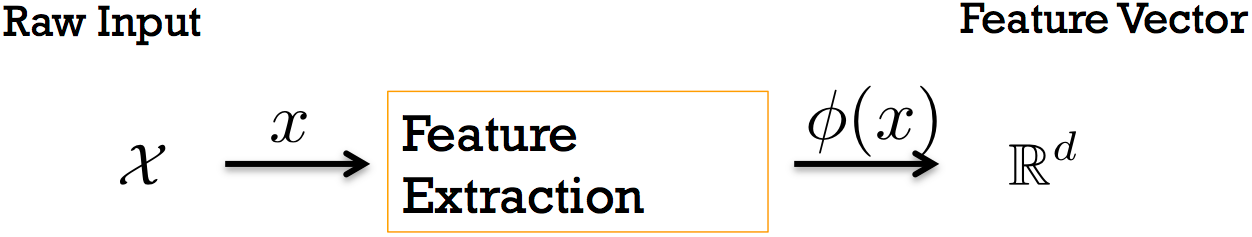
\includegraphics[width=0.9\textwidth]{../Figures/features/feature-extraction}
\par\end{center}

\end{frame}

\begin{frame}{Motivation}

\begin{itemize}
\item Two motivations for thinking about feature extraction:
	\begin{itemize}
		\item Motivation 1 -- consuming inputs that are not natively in $\reals^{d}$ -- examples?
		\begin{itemize}
		\pause{}
			\item Text documents
			\item Image files
			\item Sound recordings
			\item DNA sequences
			\pause{}
		\end{itemize}
		\item But everything in a computer is a sequence of numbers?

		\pause{}
		\begin{itemize}
			\item The $i$th entry of each sequence should have the same ``meaning''
			\item All the sequences should have the same length
		\end{itemize}
	\end{itemize}
\end{itemize}
\end{frame}



\begin{frame}
\begin{center}
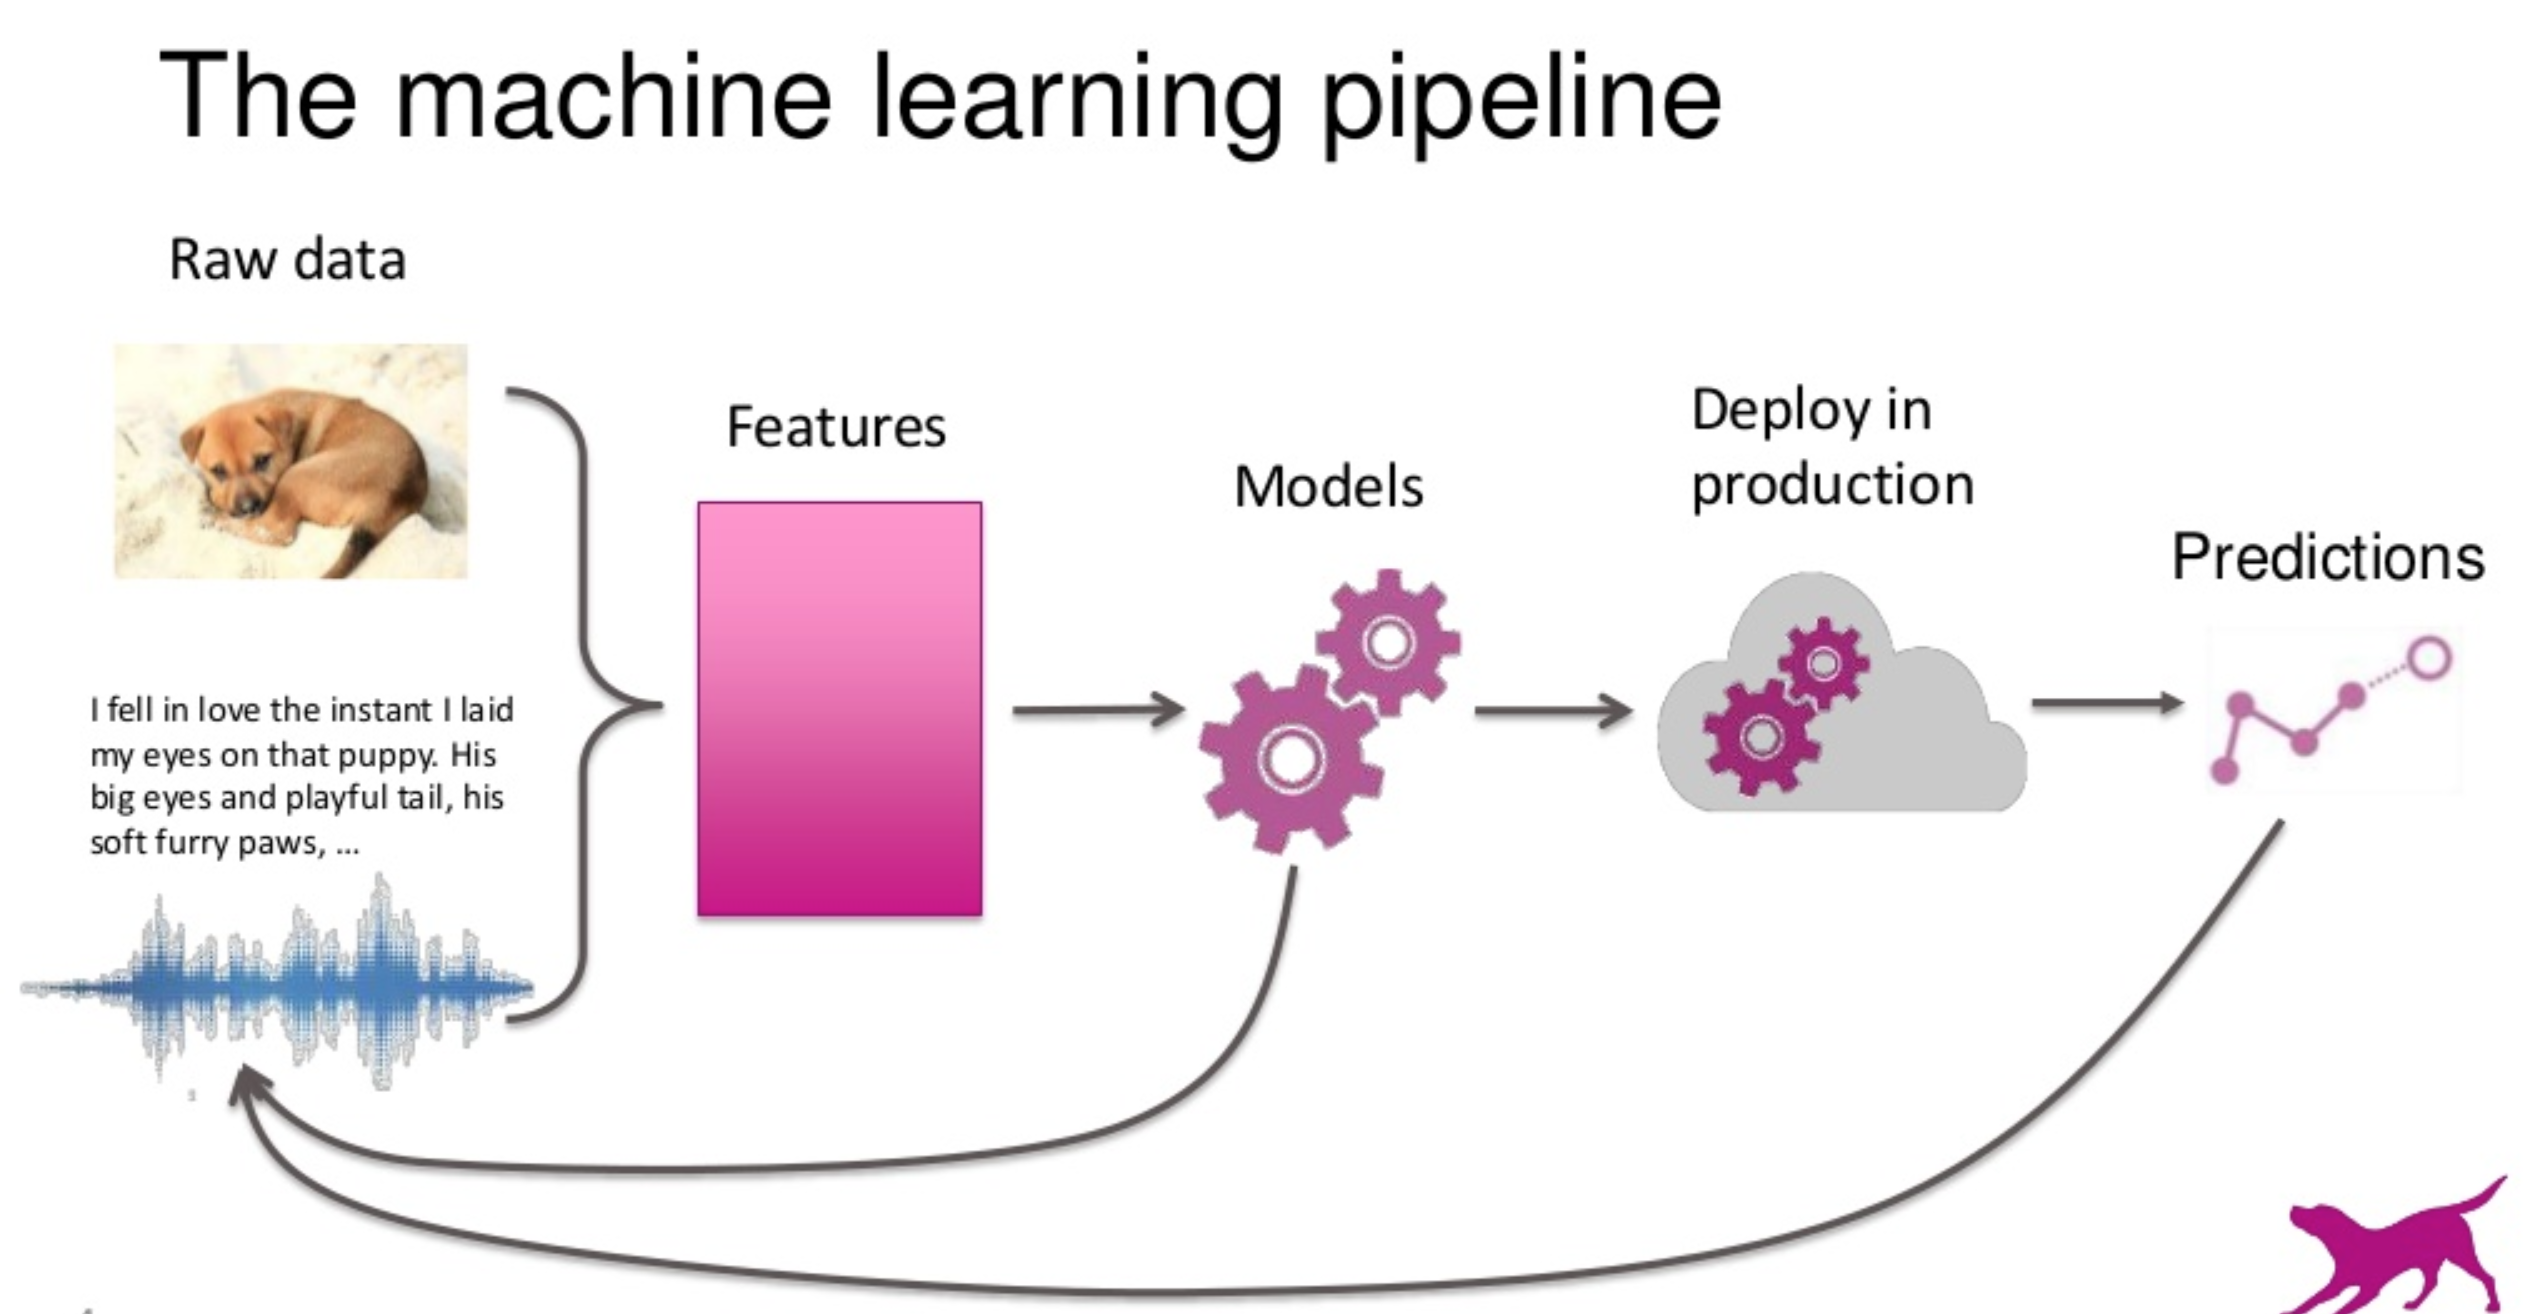
\includegraphics[width=0.9\textwidth]{../Figures/alice_zheng.png}
\par\end{center}
\let\thefootnote\relax\footnotetext{\tiny{\url{https://www.slideshare.net/AliceZheng3/understanding-feature-space-in-machine-learning}}}
\end{frame}

\section{Feature Templates}
\begin{frame}{Example: Detecting Email Addresses }

\begin{itemize}
\item Task: Predict whether a string is an email address
\end{itemize}

\pause{}
\begin{itemize}
\item Could use domain knowledge and write down:
\end{itemize}
\begin{center}
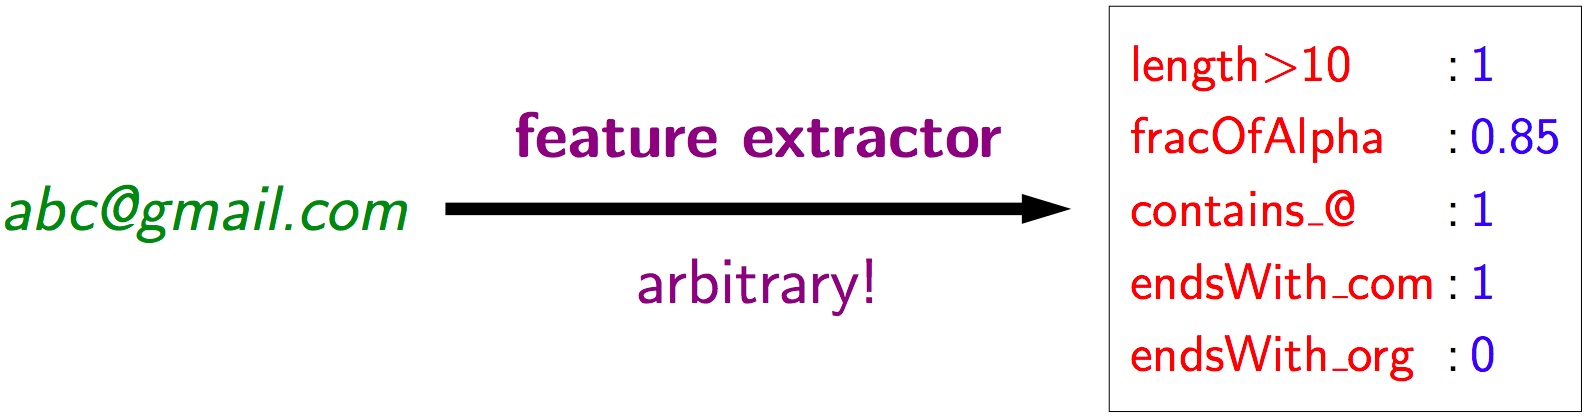
\includegraphics[width=0.75\columnwidth]{../Figures/features/emailFeatures}
\par\end{center}

\pause{}
\begin{itemize}
\item But this was ad-hoc, and maybe we missed something.
\item Could be more systematic?
\end{itemize}
\let\thefootnote\relax\footnotetext{\tiny{From Percy Liang's "Lecture 3" slides from Stanford's CS221, Autumn 2014. }}
\end{frame}

\begin{frame}{Feature Templates }

\begin{definition}
[informal]A \textbf{feature template} is a group of features all
computed in a similar way.
\end{definition}


\pause{}
\begin{itemize}
\item Input: \textsl{\textcolor{blue}{abc@gmail.com}}

\pause{}

\end{itemize}
\begin{exampleblock}{Feature Templates}
\end{exampleblock}
\begin{itemize}
\item Length greater than \_\_\_

\pause{}
\item Last three characters equal \_\_\_ 

\pause{}
\item Contains character \_\_\_
\end{itemize}
\let\thefootnote\relax\footnotetext{\tiny{Based on Percy Liang's "Lecture 3" slides from Stanford's CS221, Autumn 2014. }}
\end{frame}

\begin{frame}{Feature Template: Last Three Characters Equal \_\_\_ }
\begin{itemize}
\item Don't think about which 3-letter suffixes are meaningful...
\item Just \textbf{include them all.}

\pause{}
\end{itemize}
\begin{center}
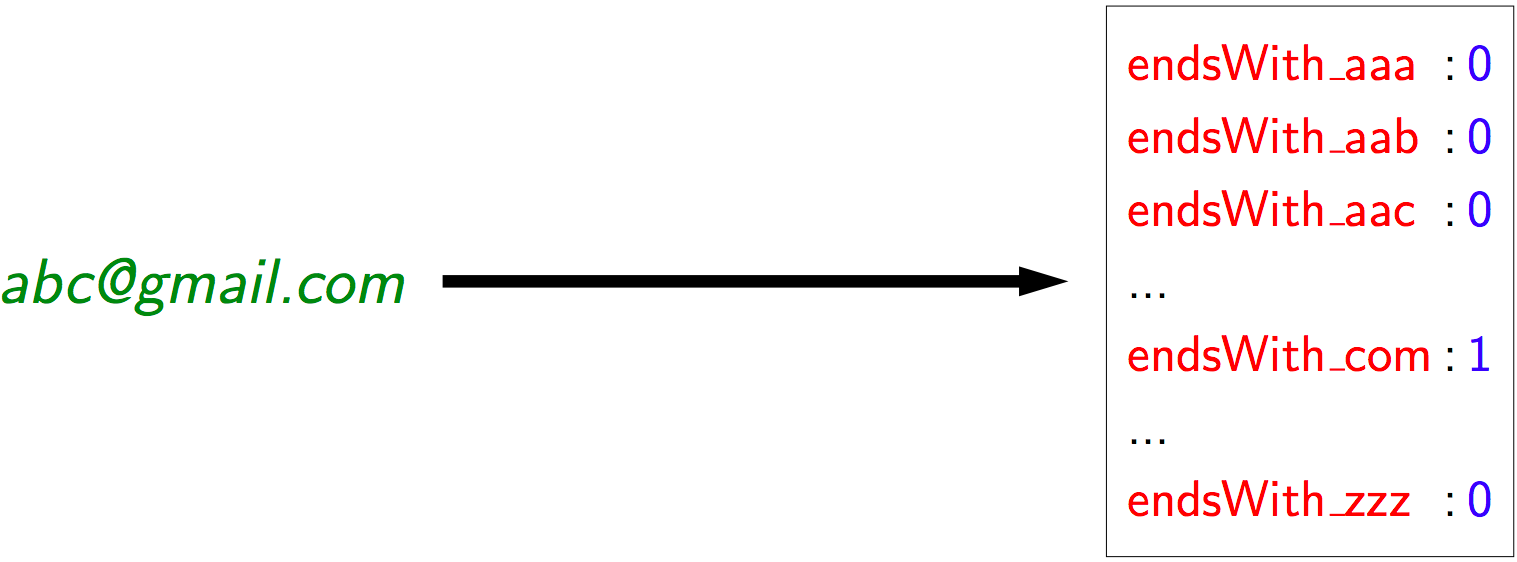
\includegraphics[width=0.75\columnwidth]{../Figures/features/last3CharactersFeature}
\par\end{center}

\pause{}
\begin{itemize}
\item With regularization, our methods will not be overwhelmed.
\end{itemize}
\let\thefootnote\relax\footnotetext{\tiny{From Percy Liang's "Lecture 3" slides from Stanford's CS221, Autumn 2014. }}
\end{frame}


\begin{frame}{Feature Vector Representations}
\begin{center}
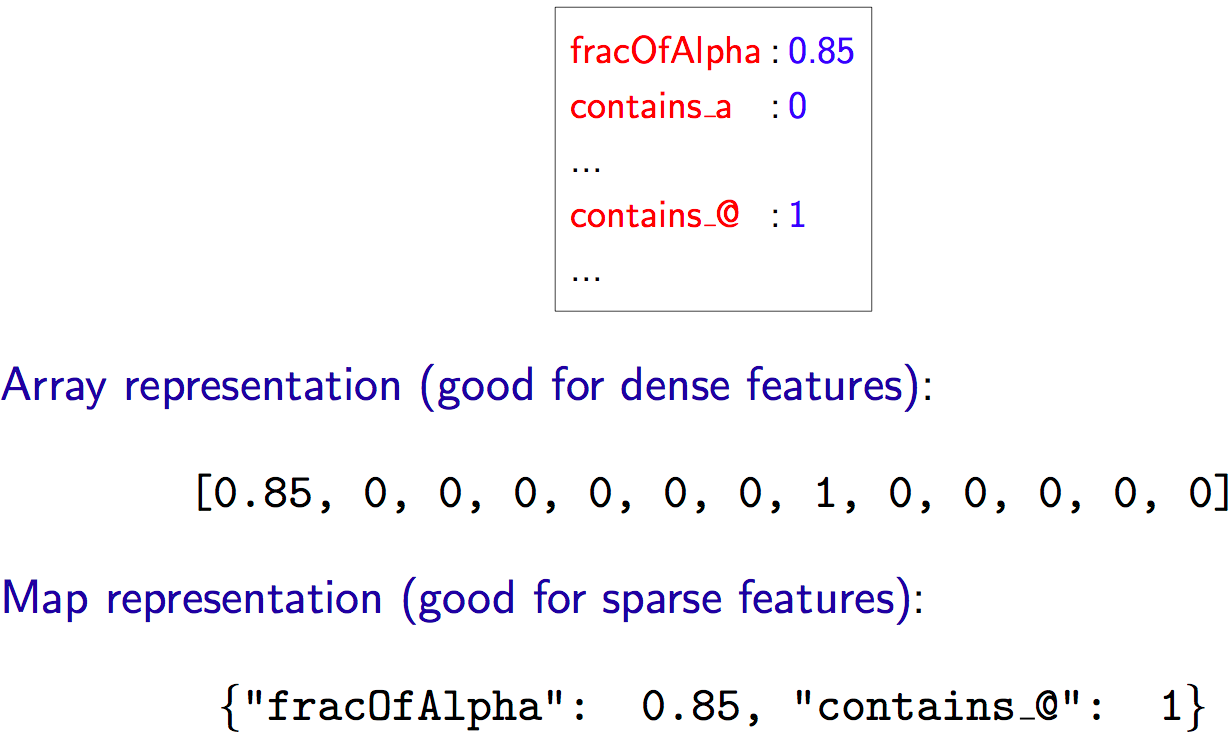
\includegraphics[height=0.7\textheight]{../Figures/features/ftrRepresentations}
\par\end{center}

\let\thefootnote\relax\footnotetext{\tiny{From Percy Liang's "Lecture 3" slides from Stanford's CS221, Autumn 2014. }}
\end{frame}

\begin{frame}{Feature Vector Representations}
\begin{itemize}
\item Arrays
\begin{itemize}
\item assumed fixed ordering of the features 

\pause{}
\item appropriate when significant number of nonzero elements\\
(``\textbf{dense feature vectors}'')

\pause{}
\item very efficient in space and speed (and you can take advantage of GPUs)

\pause{}
\end{itemize}
\item Map (a ``dict'' in Python)
\begin{itemize}
\item best for \textbf{sparse feature vectors} (i.e. few nonzero features)

\pause{}
\item features not in the map have default value of zero

\pause{}
\item Python code for ``ends with last 3 characters'': 
\begin{lyxcode}
\textcolor{black}{\{\textquotedbl{}endsWith\_\textquotedbl{}+x{[}-3:{]}:~1\}}.

\pause{}
\end{lyxcode}
\item On \texttt{\textcolor{black}{\textquotedbl{}example string\textquotedbl{}}}
we'd get \texttt{\textcolor{black}{\{\textquotedbl{}endsWith\_ing\textquotedbl{}: 1\}}}.

\pause{}
\item Has overhead compared to arrays, so much slower for dense features.
\item Question:  if we have a sparse feature vector, what are the implications for preprocessing?
\end{itemize}
\end{itemize}
\let\thefootnote\relax\footnotetext{\tiny{From Percy Liang's "Lecture 3" slides from Stanford's CS221, Autumn 2014. }}
\end{frame}


\section{Feature Map -- ingesting inputs not natively in $\reals^d$}
\begin{frame}{Example: Classifying documents from 20 newsgroups}
\begin{itemize}
\item Context: The newsgroups dataset comprises around 18000 newsgroups posts on 20 topics.
\pause{}
\item We'll restrict ourselves to classifying posts within 4 topics:
\begin{itemize}
	\item 'alt.atheism'
	\item 'soc.religion.christian'
	\item 'comp.graphics'
	\item 'sci.med'.
\end{itemize}
\item Thanks to the sklearn team for this worked example (at \url{http://scikit-learn.org/stable/tutorial/text_analytics/working_with_text_data.html}).
\let\thefootnote\relax\footnotetext{\tiny{See \url{https://github.com/davidrosenberg/mlcourse/blob/gh-pages/Notebooks/Features/test_BOW.ipynb} for this example in full.}}
\end{itemize}
\end{frame}
I
\begin{frame}{Example: Classifying documents from 20 newsgroups}
\textbf{Example Document}:
\begin{center}
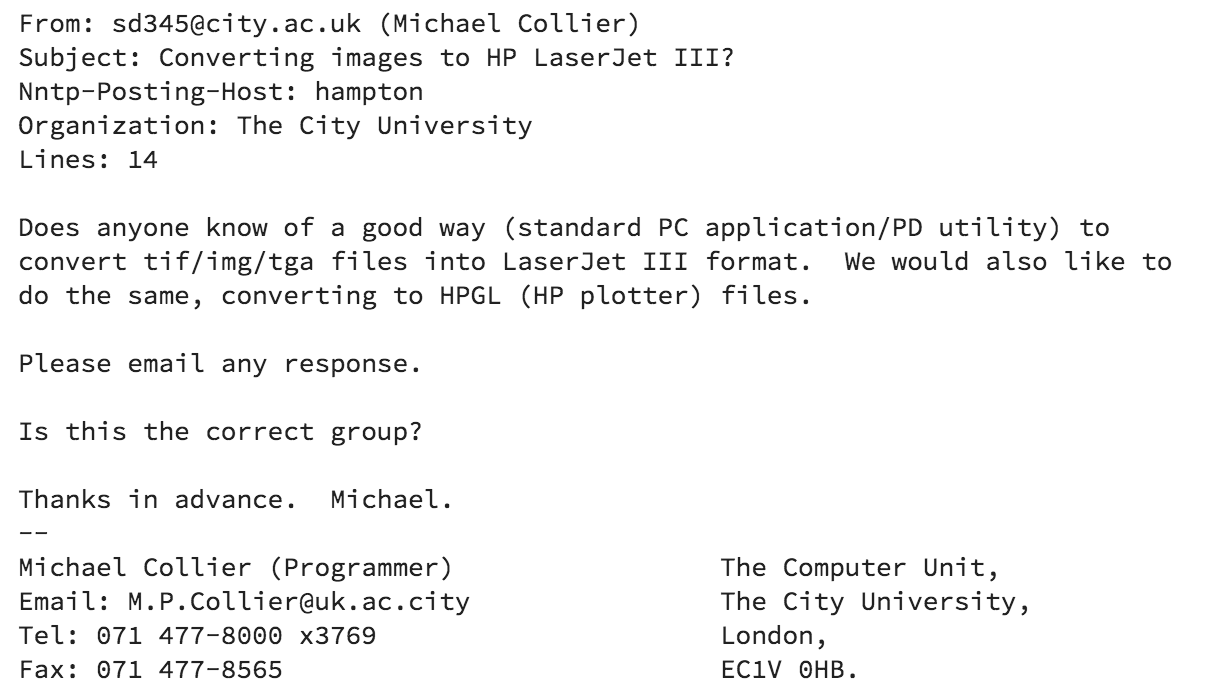
\includegraphics[height=0.8\textheight]{../Figures/first_doc.png}
\par\end{center}
\end{frame}


\begin{frame}{Example: Classifying documents from 20 newsgroups}
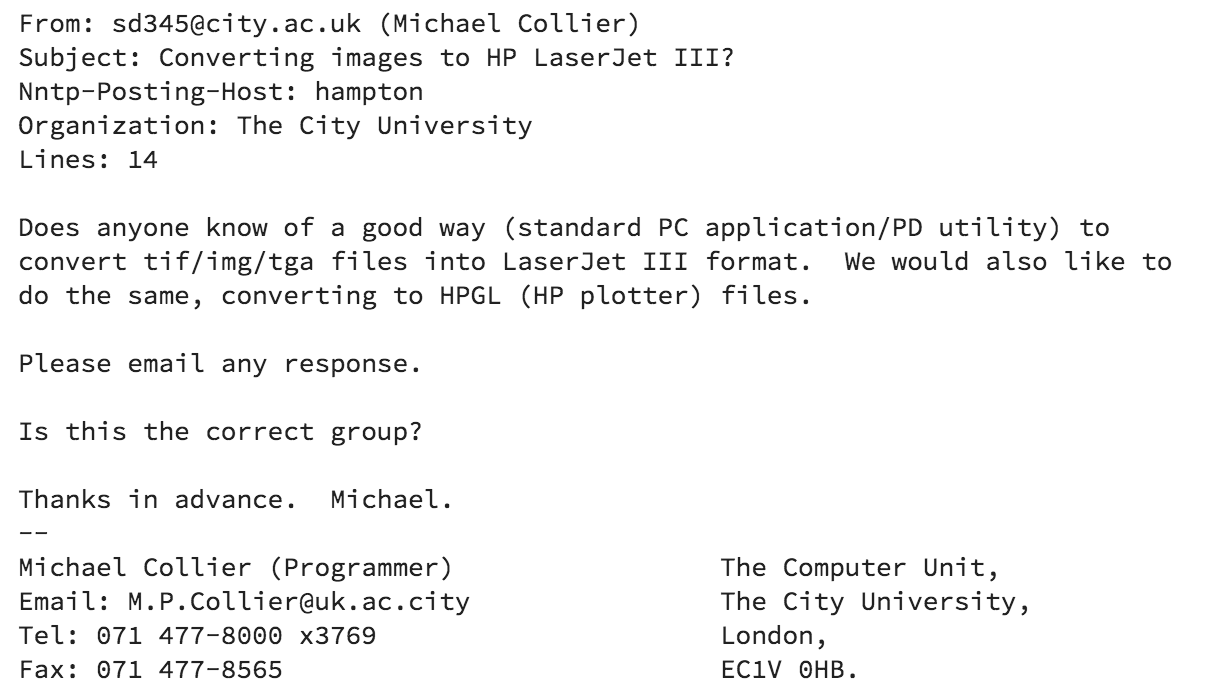
\includegraphics[height=0.4\textheight,trim={0 5cm 0 0},clip]{../Figures/first_doc.png}
\begin{itemize}
	\item What feature maps could we apply over these sorts of documents?
	\pause{}
	\item A simple approach -- bag-of-words (BOW). 
	\begin{itemize}
		\item Assign a fixed integer id to each word occurring in any document of the training set.
		\item For each document $i$, count the number of occurrences of each word $w$ and store it (sparsely) as $doc_i[w] = j_w$ == count of word $w$ in document $i$.
		\item The BOW representation implies that $n_{features}$ is the number of distinct words in the corpus.
		\item What is the feature map $\phi(x)$?
		\pause{}
		\item $\phi(x) = [j_{word_{1}},\cdots,j_{word_{n_{words}}}]$
	\end{itemize}
\end{itemize}
\end{frame}


\begin{frame}{Example: Classifying documents from 20 newsgroups}
\begin{itemize}
	\item Here's the classifier we'll fit (note we're adding the \texttt{TfidfTransformer} to scale by inverse document frequency, since it improves performance on this task -- if you're not familiar with TF-IDF see the docs).
\end{itemize}
\begin{center}
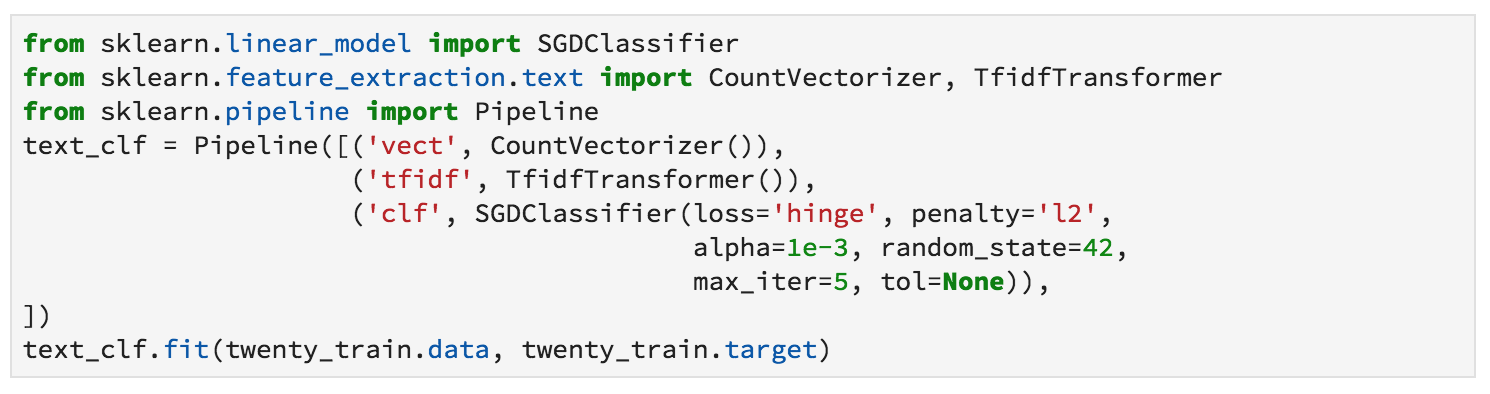
\includegraphics[width=0.9\textwidth]{../Figures/bow_clf.png}
\begin{itemize}
	\item Which named steps in this Pipeline comprise our feature map $\phi$?
\end{itemize}
\par\end{center}

\end{frame}

\begin{frame}{Example: Classifying documents from 20 newsgroups}
\begin{center}
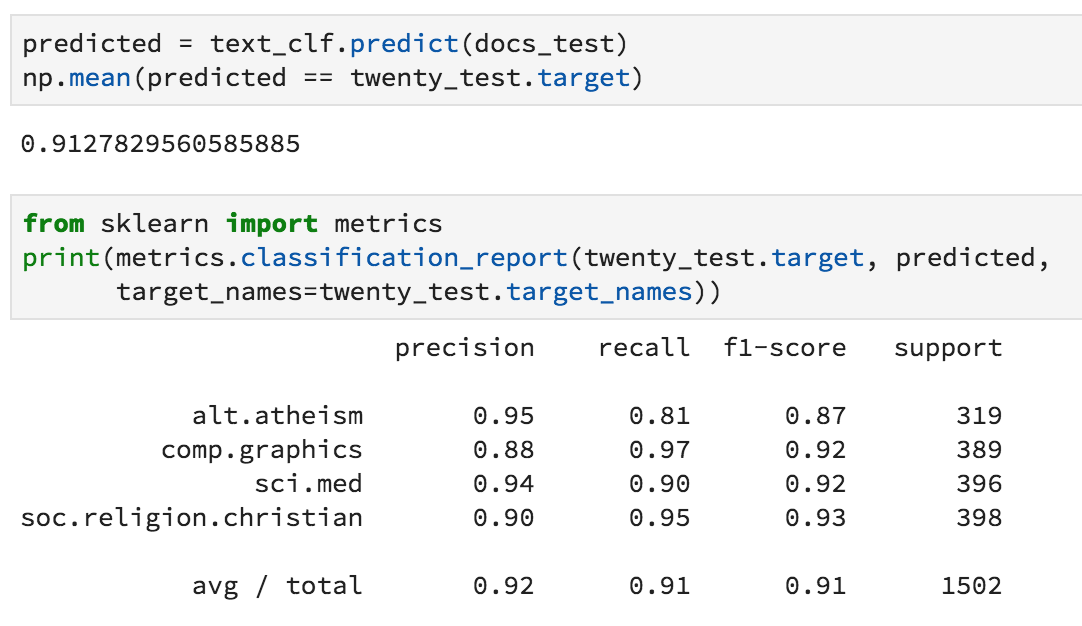
\includegraphics[width=0.7\textwidth]{../Figures/bow_clf_performance.png}
\begin{itemize}
	\item Key takeaway: need feature map  $\phi$ when dealing with inputs not natively in $\reals^d$.
\end{itemize}
\par\end{center}

\end{frame}



\begin{frame}{Motivation}
\begin{itemize}
\item Two motivations for thinking about feature extraction:
\begin{itemize}
	\item Motive 2 -- Improving performance. Think about HW2.
	\end{itemize}
\end{itemize}
\begin{center}
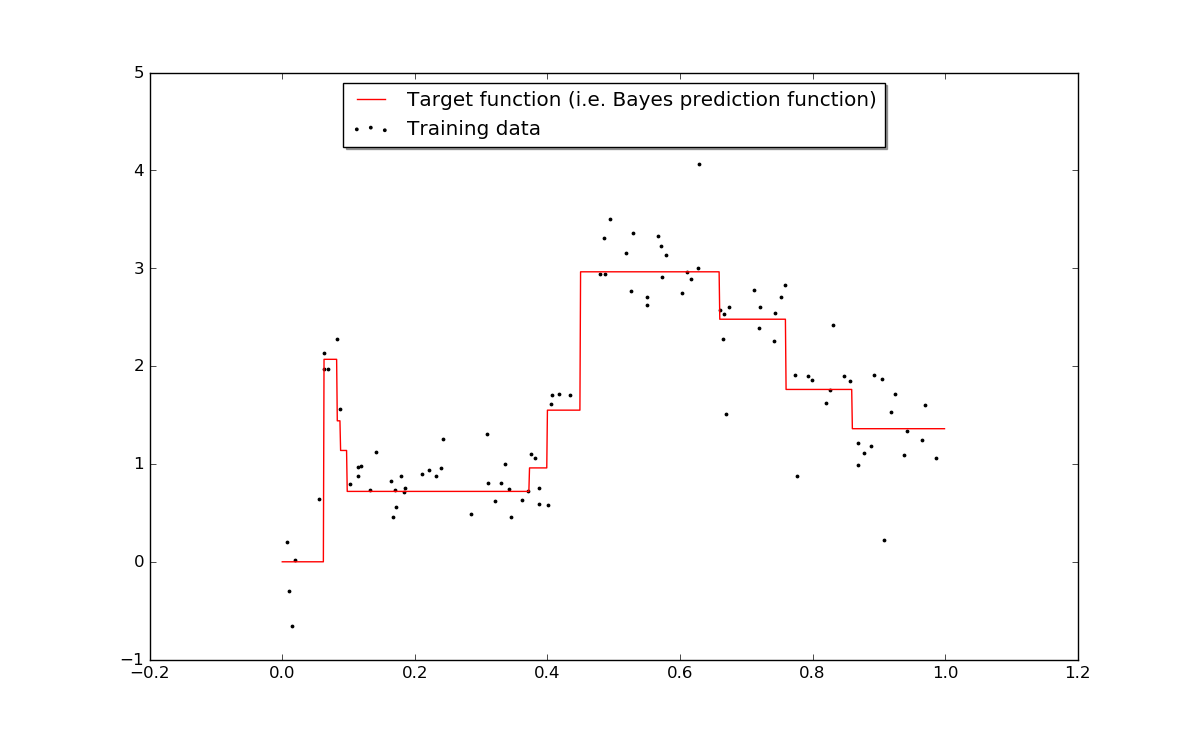
\includegraphics[width=0.5\textwidth]{../Figures/training-data-and-target-fn.png}
\par\end{center}
\begin{itemize}
	\item What was our feature map $\phi(x)$? $\phi(x) \in \reals^k$ for what $k$?
	\pause{}
	\item $\phi(x) = \left[\mathbbm{1}(x \geq \frac{1}{400}), \cdots,\mathbbm{1}(x \geq \frac{399}{400}) \right]$
\end{itemize}
\end{frame}

\begin{frame}{Motivation}
\begin{itemize}
\item Two motivations for thinking about feature extraction:
\begin{itemize}
	\item Motive 2 -- Improving performance. Think about HW2.
	\end{itemize}
\end{itemize}
\begin{center}
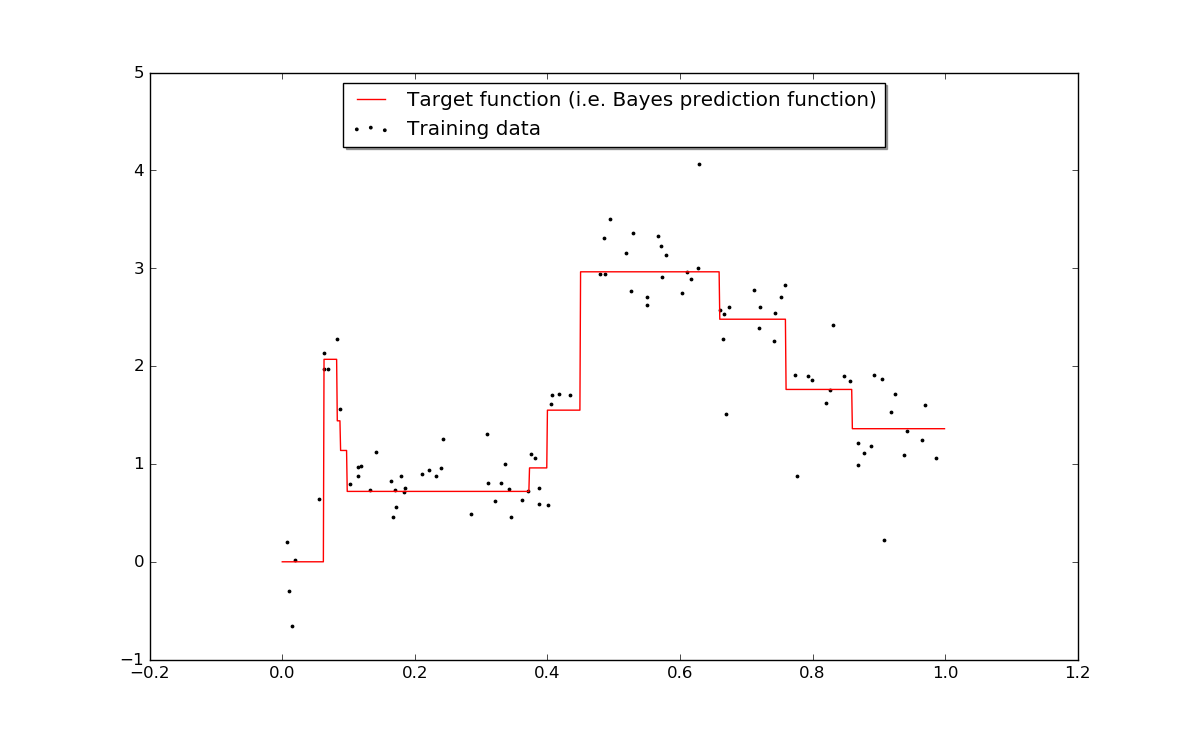
\includegraphics[width=0.5\textwidth]{../Figures/training-data-and-target-fn.png}
\par\end{center}
\begin{itemize}
	\item Why did we use this feature map instead of just learning a prediction function $y\sim x$?
\end{itemize}
\end{frame}


\begin{frame}{Motivation}
\begin{itemize}
\item Two motivations for thinking about feature extraction:
\begin{itemize}
	\item Motive 2 -- Improving performance. Toy Example:
	\end{itemize}
\end{itemize}
\begin{center}
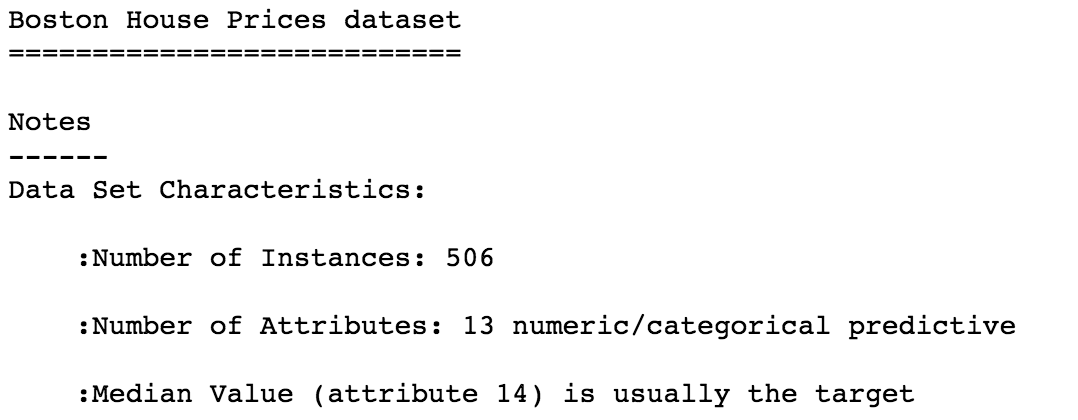
\includegraphics[width=0.9\textwidth]{../Figures/boston_DESCR.png}
\par\end{center}
\end{frame}


\begin{frame}{Motivation}
\begin{itemize}
\item Two motivations for thinking about feature extraction:
\begin{itemize}
	\item Motive 2 -- Improving performance. Toy Example:
\end{itemize}
\end{itemize}
\begin{center}
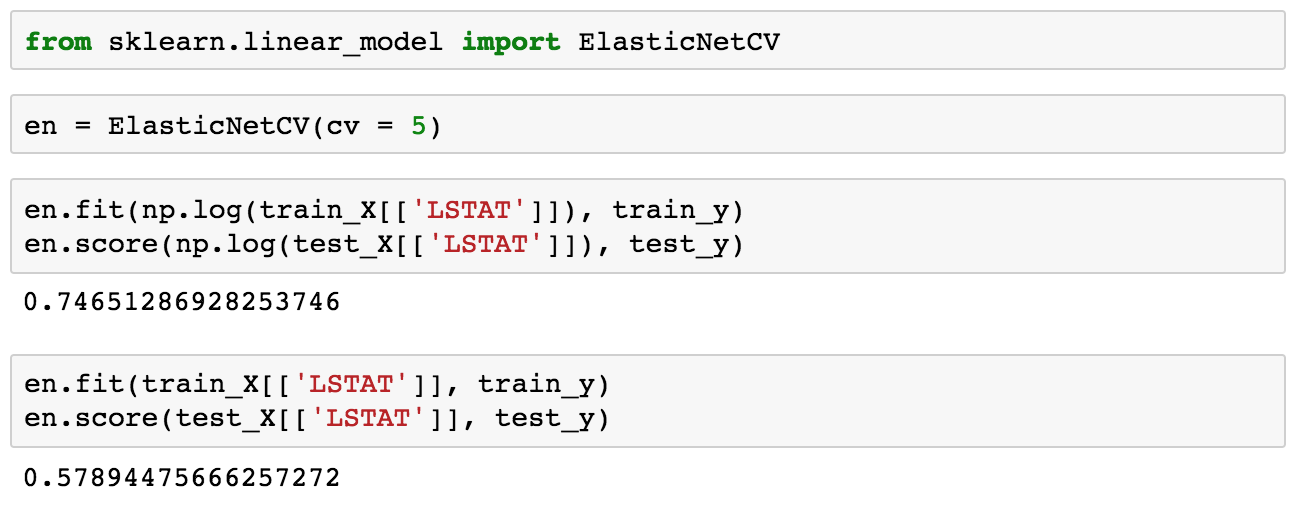
\includegraphics[width=0.7\textwidth]{../Figures/boston_toy_ex.png}
\par\end{center}
\let\thefootnote\relax\footnotetext{\tiny{See \url{https://github.com/davidrosenberg/mlcourse/blob/gh-pages/Notebooks/Features/simple_feature_transformations.ipynb}}}
\end{frame}

\begin{frame}{Motivation}
\begin{itemize}
\item We'll be looking at regression examples throughout this lab.
\item Using Elastic Net in sklearn, the default score method returns the coefficient of determination $R^2$ of the prediction.
\item Recall:
\end{itemize}
\begin{center}
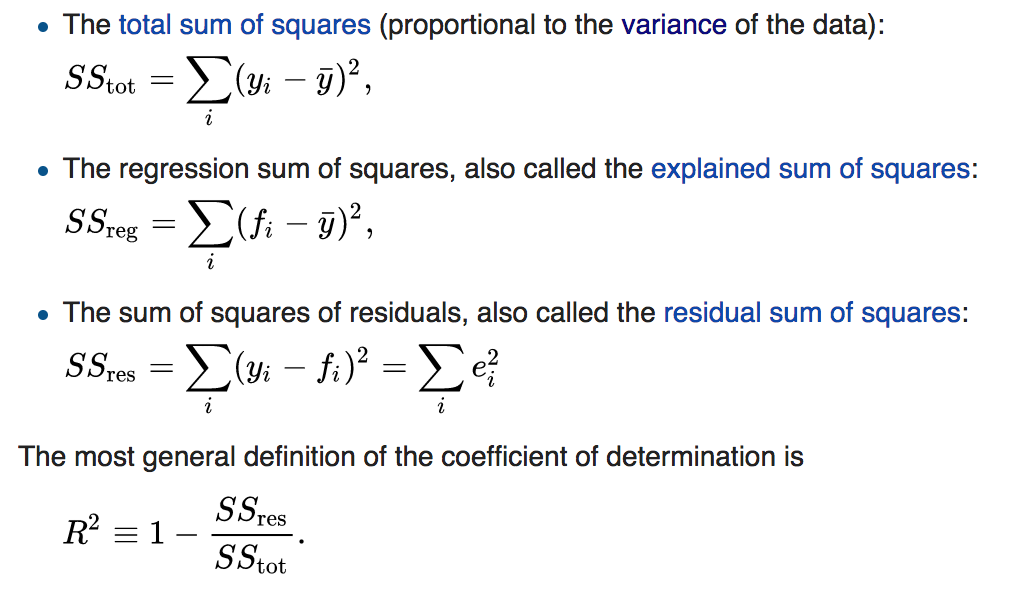
\includegraphics[width=0.6\textwidth]{../Figures/r_2_reminder.png}
\par\end{center}
\end{frame}


\begin{frame}{Motivation}
\begin{itemize}
\item Key idea: instead of using more flexible (i.e. non-linear) models, build better features.
\end{itemize}
\begin{tabular}{l r}
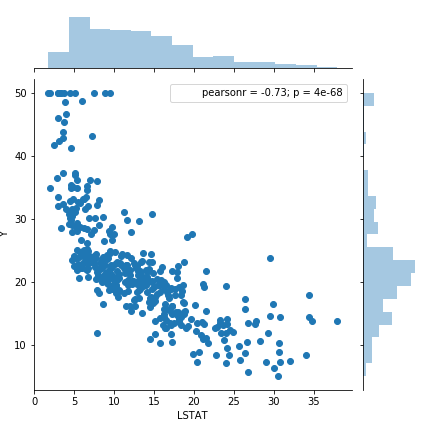
\includegraphics[width=0.4\textwidth]{../Figures/untransformed_lstat.png} &
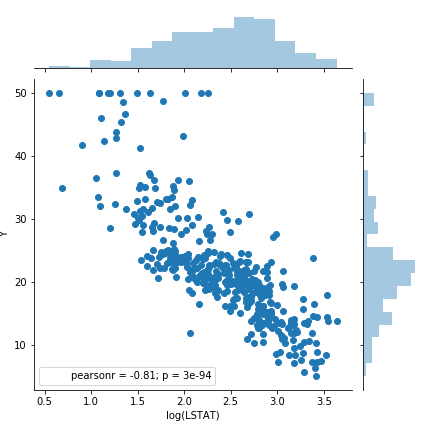
\includegraphics[width=0.4\textwidth]{../Figures/transformed_lstat.png}
\end{tabular}
\end{frame}

\section{Handling Nonlinearity with Linear Methods}
\begin{frame}{Example Task: Predicting Health}
\begin{itemize}
\item General Philosophy: Extract every feature that might be relevant

\pause{}
\item Features for medical diagnosis
\begin{itemize}
\item height
\item weight
\item body temperature
\item blood pressure
\item etc...
\end{itemize}
\end{itemize}
\let\thefootnote\relax\footnotetext{\tiny{From Percy Liang's "Lecture 3" slides from Stanford's CS221, Autumn 2014. }}
\end{frame}

\begin{frame}{Issues for Linear Predictors}
\begin{itemize}
\item For linear predictors, it's important \textbf{how} features are added

\pause{}
\item Three types of nonlinearities can cause problems:

\pause{}
\begin{enumerate}
\item Non-monotonicity
\item Saturation
\item Interactions between features
\end{enumerate}
\end{itemize}
\let\thefootnote\relax\footnotetext{\tiny{From Percy Liang's "Lecture 3" slides from Stanford's CS221, Autumn 2014. }}
\end{frame}

\begin{frame}{Non-monotonicity: The Issue}
\begin{itemize}
\item Feature Map: $\phi(x)=\left[1,\text{temperature}(x)\right]$

\pause{}
\item Action: Predict health score $y\in\reals$ (positive is good)

\pause{}
\item Hypothesis Space $\cf=\left\{ \mbox{affine functions of temperature}\right\} $

\pause{}
\item Issue: 

\pause{}
\begin{itemize}
\item Health is not an affine function of temperature.

\pause{}
\end{itemize}
\item Affine function can either say
\begin{itemize}
\item Very high is bad and very low is good, or
\item Very low is bad and very high is good,
\item But here, both extremes are bad.
\end{itemize}
\end{itemize}
\let\thefootnote\relax\footnotetext{\tiny{From Percy Liang's "Lecture 3" slides from Stanford's CS221, Autumn 2014. }}
\end{frame}

\begin{frame}{Non-monotonicity: Solution 1}
\begin{itemize}
\item Transform the input:
\[
\phi(x)=\left[1,\left\{ \text{temperature(x)-37}\right\} ^{2}\right],
\]
where $37$ is ``normal'' temperature in Celsius.

\pause{}
\item Ok, but this requires domain knowledge 
\begin{itemize}
\item Do we really need that?
\end{itemize}
\end{itemize}
\let\thefootnote\relax\footnotetext{\tiny{From Percy Liang's "Lecture 3" slides from Stanford's CS221, Autumn 2014. }}
\end{frame}

\begin{frame}{Non-monotonicity: Solution 2}
\begin{itemize}
\item Think less, put in more:
\[
\phi(x)=\left[1,\text{temperature}(x),\left\{ \text{temperature}(x)\right\} ^{2}\right].
\]


\pause{}
\item \textbf{More expressive} than Solution 1.

\pause{}

\end{itemize}
\begin{block}{General Rule}

Features should be simple building blocks that can be pieced together.
\end{block}
\let\thefootnote\relax\footnotetext{\tiny{From Percy Liang's "Lecture 3" slides from Stanford's CS221, Autumn 2014. }}
\end{frame}

\begin{frame}{Saturation: The Issue}
\begin{itemize}
\item Setting: Find products relevant to user's query

\pause{}
\item Input: Product $x$
\item Action: Score the relevance of $x$ to user's query

\pause{}
\item Feature Map:
\[
\phi(x)=\left[1,N(x)\right],
\]
where $N(x)=\text{number of people who bought }x$.

\pause{}
\item We expect a monotonic relationship between $N(x)$ and relevance,
but...
\end{itemize}
\let\thefootnote\relax\footnotetext{\tiny{From Percy Liang's "Lecture 3" slides from Stanford's CS221, Autumn 2014. }}
\end{frame}

\begin{frame}{Saturation: The Issue}
\begin{alertblock}{Is relevance linear in N(x)?}
\begin{itemize}
\item Relevance score reflects confidence in relevance prediction.
\item Are we 10 times more confident if $N(x)=1000$ vs $N(x)=100$?

\pause{}
\end{itemize}
\end{alertblock}
\begin{itemize}
\item Bigger is better... but not that much better. 
\end{itemize}
\let\thefootnote\relax\footnotetext{\tiny{From Percy Liang's "Lecture 3" slides from Stanford's CS221, Autumn 2014. }}
\end{frame}

\begin{frame}{Saturation: Solve with nonlinear transform}
\begin{itemize}
\item Smooth nonlinear transformation:
\[
\phi(x)=\left[1,\log\left\{ 1+N(x)\right\} \right]
\]


\pause{}
\item $\log\left(\cdot\right)$ good for values with large dynamic ranges

\pause{}
\item \emph{Does it matter what base we use in the log?}
\end{itemize}
\let\thefootnote\relax\footnotetext{\tiny{From Percy Liang's "Lecture 3" slides from Stanford's CS221, Autumn 2014. }}
\end{frame}

\begin{frame}{Saturation: Solve by discretization}
\begin{itemize}
\item Discretization (a discontinuous transformation):
\[
\phi(x)=\left(\ind{5\le N(x)<10},\ind{10\le N(x)<100},\ind{100\le N(x)}\right)
\]


\pause{}
\item Sometimes we might prefer one-sided buckets 
\[
\phi(x)=\left(\ind{5\le N(x)},\ind{10\le N(x)},\ind{100\le N(x)}\right)
\]

\begin{itemize}
\item Why? $\pause$Hint: What's the effect of regularization on the parameters
for rare buckets? 
\end{itemize}

\pause{}
\item Small buckets allow quite flexible relationship
\end{itemize}
\end{frame}

\begin{frame}{Interactions: The Issue}
\begin{itemize}
\item Input: Patient information $x$
\item Action: Health score $y\in\reals$ (higher is better)
\item Feature Map
\[
\phi(x)=\left[\mbox{height}(x),\mbox{weight}(x)\right]
\]


\pause{}
\item Issue: It's the weight \textbf{relative} to the height that's important.

\pause{}
\item Impossible to get with these features and a linear classifier.
\item Need some \textbf{interaction} between height and weight.

\let\thefootnote\relax\footnotetext{\tiny{From Percy Liang's "Lecture 3" slides from Stanford's CS221, Autumn 2014. }}
\end{itemize}
\end{frame}

\begin{frame}{Interactions: Approach 1}
\begin{itemize}
\item Google ``ideal weight from height''

\pause{}
\item J. D. Robinson's ``ideal weight'' formula (for a male):
\[
\mbox{weight}\mbox{(kg)}=52+1.9\left[\mbox{height(in)}-60\right]
\]


\pause{}
\item Make score square deviation between height($h$) and ideal weight($w$)
\[
f(x)=\left(52+1.9\left[h(x)-60\right]-w(x)\right)^{2}
\]


\pause{}
\item WolframAlpha for complicated Mathematics:
\[
f(x)=3.61h(x)^{2}-3.8h(x)w(x)-235.6h(x)+w(x)^{2}+124w(x)+3844
\]
\end{itemize}
\let\thefootnote\relax\footnotetext{\tiny{From Percy Liang's "Lecture 3" slides from Stanford's CS221, Autumn 2014. }}
\end{frame}

\begin{frame}{Interactions: Approach 2}
\begin{itemize}
\item Just include all second order features:
\[
\phi(x)=\left[1,h(x),w(x),h(x)^{2},w(x)^{2},\underbrace{h(x)w(x)}_{\mbox{cross term}}\right]
\]


\pause{}
\item More flexible, no Google, no WolframAlpha.

\pause{}

\end{itemize}
\begin{block}{General Principle}

Simpler building blocks replace a single ``smart'' feature.
\end{block}
\let\thefootnote\relax\footnotetext{\tiny{From Percy Liang's "Lecture 3" slides from Stanford's CS221, Autumn 2014. }}
\end{frame}

\begin{frame}{Predicate Features and Interaction Terms}
\begin{definition}
A \textbf{predicate} on the input space $\cx$ is a function $P:\cx\to\left\{ \mbox{True},\mbox{False}\right\} $.

\pause{}
\end{definition}

\begin{itemize}
\item Many features take this form:
\begin{itemize}
\item $x\mapsto s(x)=\ind{\mbox{subject is sleeping}}$
\item $x\mapsto d(x)=\ind{\mbox{subject is driving}}$

\pause{}
\end{itemize}
\item For predicates, interaction terms correspond to \textbf{AND} conjunctions:
\begin{itemize}
\item $x\mapsto s(x)d(x)=\ind{\mbox{subject is sleeping AND subject is driving}}$
\end{itemize}
\end{itemize}
\end{frame}

\begin{frame}{So What's Linear?}
\begin{itemize}
\item Non-linear feature map $\phi:\cx\to\reals^{d}$
\item Hypothesis space:
\[
\cf=\left\{ f(x)=w^{T}\phi(x)\mid w\in\reals^{d}\right\} .
\]


\pause{}
\item Linear in $w$? Yes.

\pause{}
\item Linear in $\phi(x)$? Yes.

\pause{}
\item Linear in $x$? No.
\begin{itemize}
\item Linearity not even defined unless $\cx$ is a vector space
\end{itemize}
\end{itemize}
\begin{block}{Key Idea: Non-Linearity}
\end{block}
\begin{itemize}
\item Nonlinear $f(x)$ is important for \textbf{expressivity}. 

\pause{}
\item $f(x)$ linear in $w$ and $\phi(x)$: makes finding $f^{*}(x)$ much
easier
\end{itemize}
\let\thefootnote\relax\footnotetext{\tiny{From Percy Liang's "Lecture 3" slides from Stanford's CS221, Autumn 2014. }}
\end{frame}

\begin{frame}{Geometric Example: Two class problem, nonlinear boundary}
\begin{center}
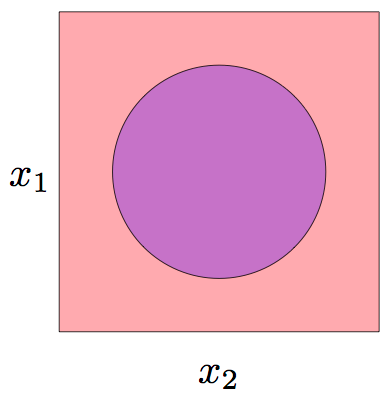
\includegraphics[height=0.5\textheight]{../Figures/features/circularBoundary}
\par\end{center}
\begin{itemize}
\item With linear feature map $\phi(x)=\left(x_{1},x_{2}\right)$ and linear
models, no hope

\pause{}
\item With appropriate nonlinearity $\phi(x)=\left(x_{1},x_{2},x_{1}^{2}+x_{2}^{2}\right)$,
piece of cake. 

\pause{}
\item Video: \url{http://youtu.be/3liCbRZPrZA} 
\end{itemize}
\let\thefootnote\relax\footnotetext{\tiny{From Percy Liang's "Lecture 3" slides from Stanford's CS221, Autumn 2014. }}
\end{frame}

\begin{frame}{Expressivity of Hypothesis Space}
\begin{itemize}
\item Consider a linear hypothesis space with a feature map $\phi:\cx\to\reals^{d}$:
\[
\cf=\left\{ f(x)=w^{T}\phi(x)\right\} 
\]


\pause{}
\end{itemize}
\begin{center}
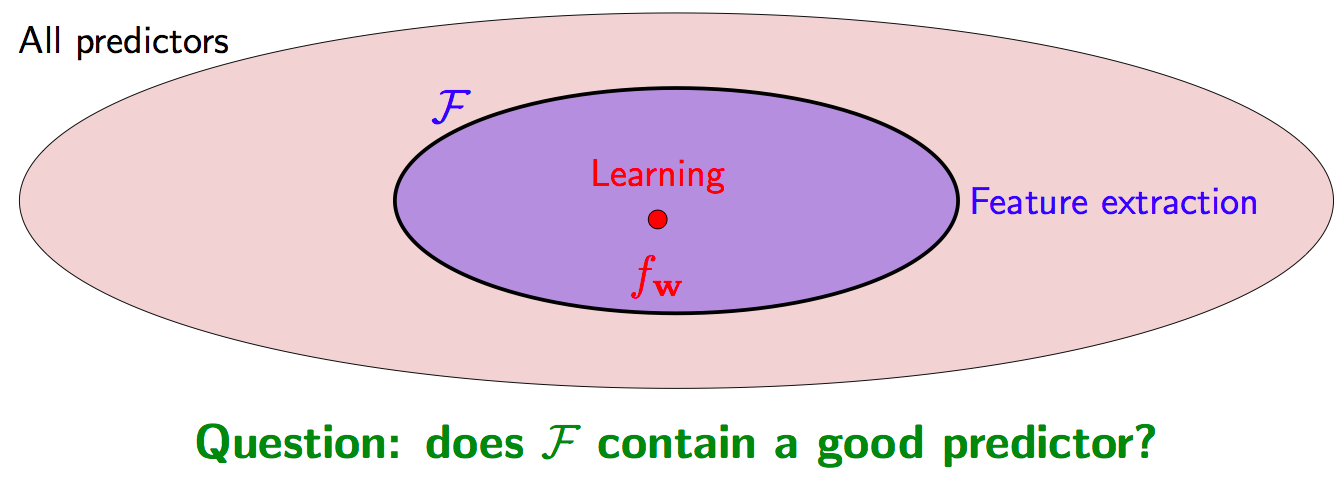
\includegraphics[width=0.75\columnwidth]{../Figures/features/featuresMakeHypothesisSpace} 
\par\end{center}

We can grow the linear hypothesis space $\cf$ by adding more features.

\let\thefootnote\relax\footnotetext{\tiny{From Percy Liang's "Lecture 3" slides from Stanford's CS221, Autumn 2014. }}
\end{frame}

\section{Example 1: Boston housing and Abalone}

\begin{frame}{Boston Housing}
\begin{itemize}
	\item Let's revisit the Boston housing dataset from the start of lab.
	\item We're going to be predicting the median house values in Boston suburbs.
	\item We'll build our feature map using \texttt{sklearn} and \texttt{sklearn\_pandas}
\end{itemize}
\begin{center}
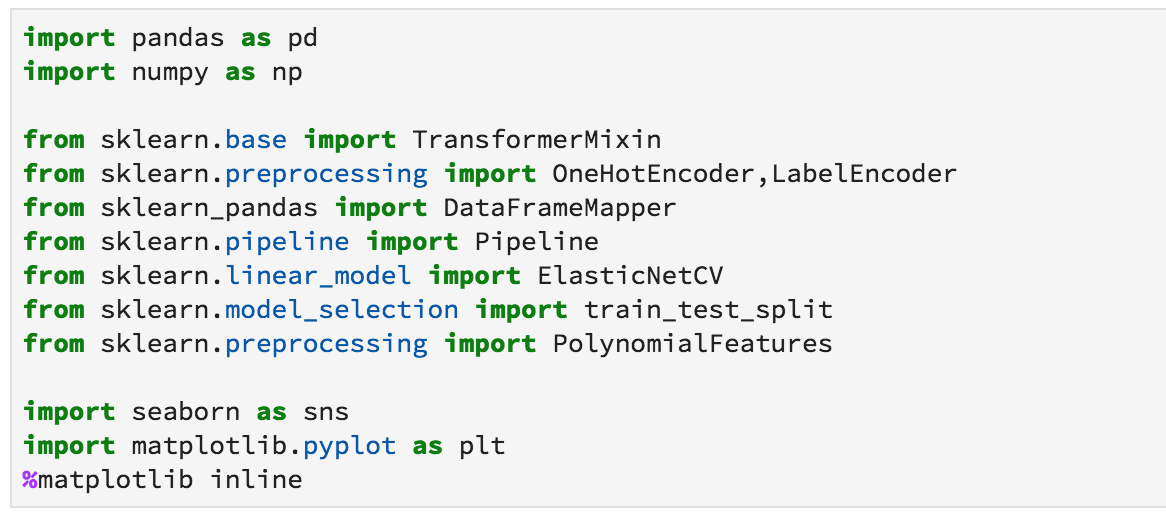
\includegraphics[width=0.75\columnwidth]{../Figures/boston_dependencies} 
\par\end{center}
\end{frame}


\begin{frame}{Boston Housing}
\begin{itemize}
	\item Set up data:
\end{itemize}
\begin{center}
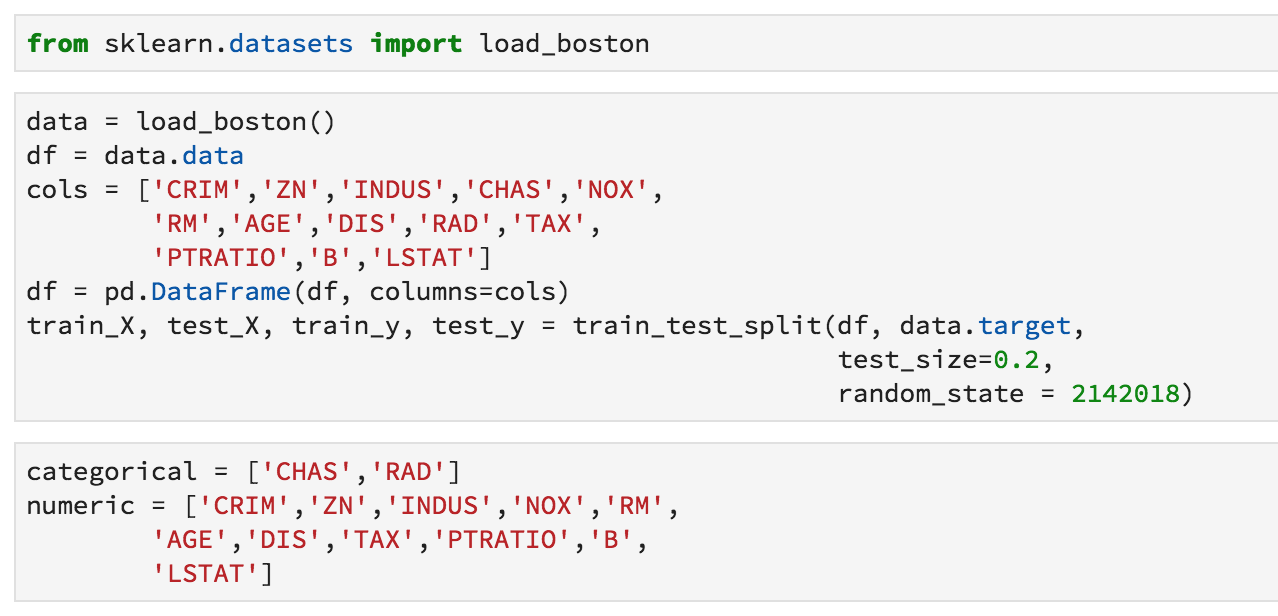
\includegraphics[width=0.65\columnwidth]{../Figures/boston_setup.png} 
\par\end{center}
\let\thefootnote\relax\footnotetext{\tiny{See \url{https://github.com/davidrosenberg/mlcourse/blob/gh-pages/Notebooks/Features/polynomial_feature_comparison.ipynb}}}
\end{frame}

\begin{frame}{Boston Housing}
\begin{itemize}
	\item Feature map 1-- looking at the code, what is the feature map $\phi_1$?
\end{itemize}
\begin{center}
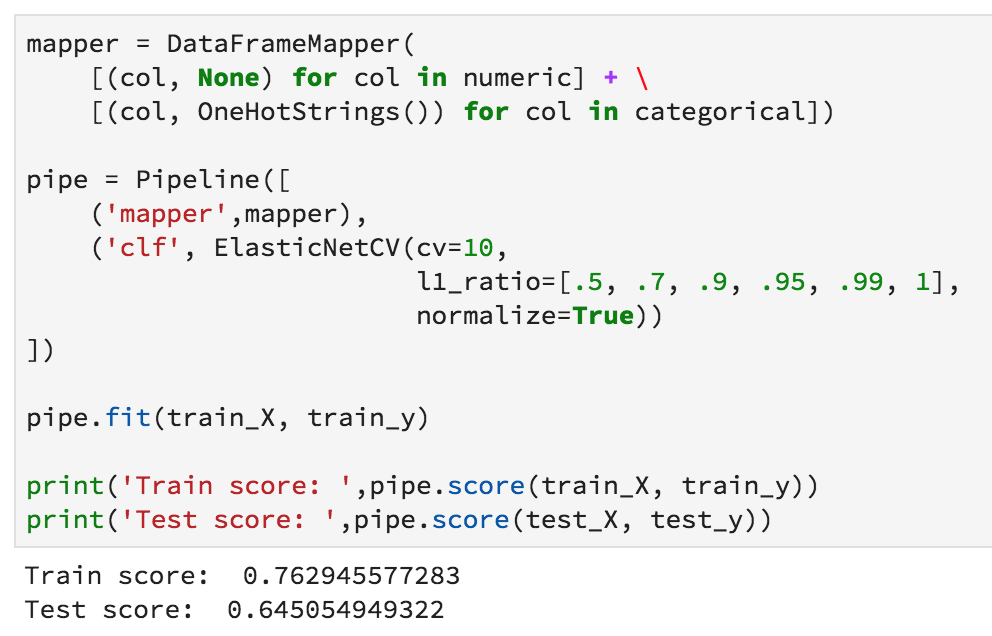
\includegraphics[width=0.55\columnwidth]{../Figures/boston_map1.png} 
\par\end{center}
\pause{}
\begin{itemize}
	\item $\phi_1(X)$ dummy encodes categoricals and passes numeric features untouched.
\end{itemize}
\end{frame}

\begin{frame}{Boston Housing}
\begin{itemize}
	\item Feature map 2-- looking at the code, what is the feature map $\phi_2$?
\end{itemize}
\begin{center}
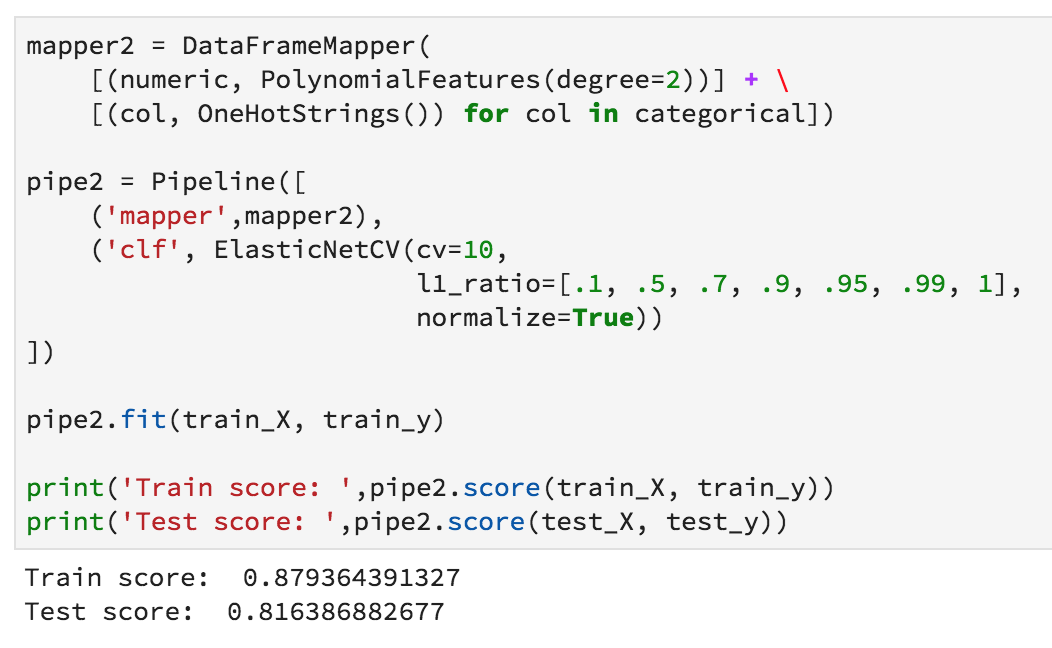
\includegraphics[width=0.55\columnwidth]{../Figures/boston_map2.png} 
\par\end{center}
\pause{}
\begin{itemize}
	\item $\phi_2(X)$ dummy encodes categoricals and maps numeric features to polynomial features of degree $d \leq 2$.
\end{itemize}
\end{frame}



\begin{frame}{Abalone}
\begin{itemize}
	\item Here we are using the abalone dataset -- predicting the number of rings on an abalone (a kind of shellfish).
	\item Set up data:
\end{itemize}
\begin{center}
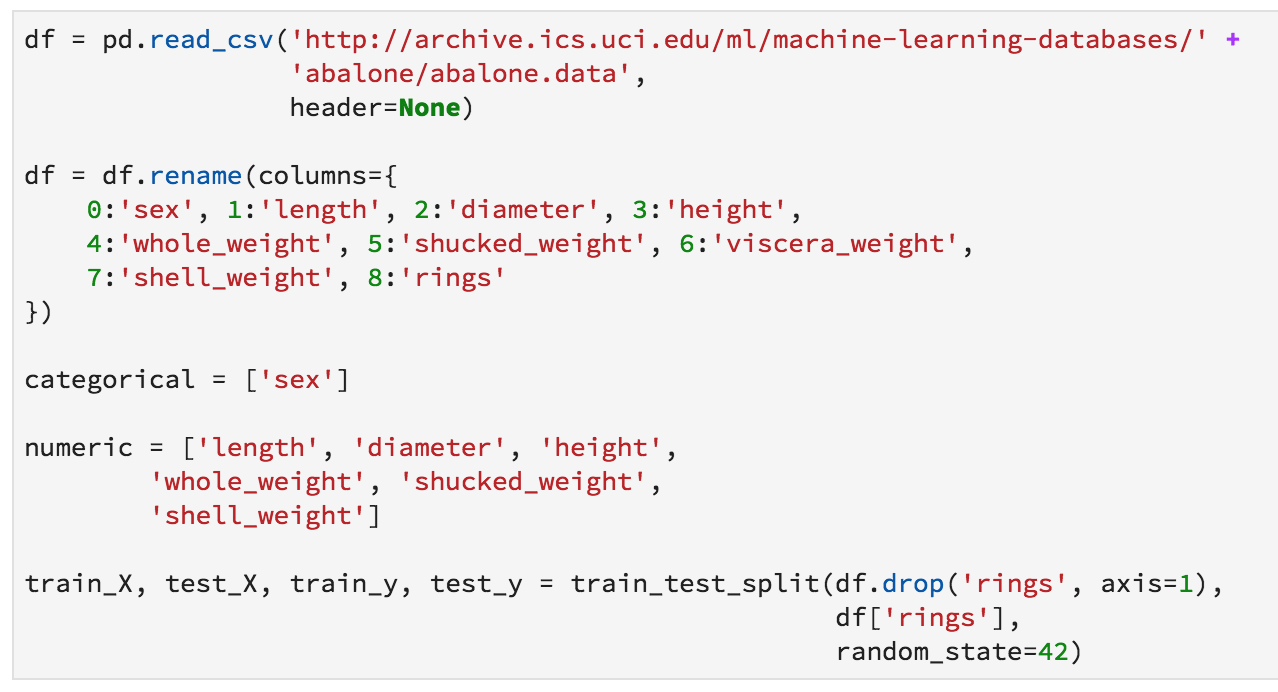
\includegraphics[width=0.6\columnwidth]{../Figures/abalone_setup.png} 
\par\end{center}
\let\thefootnote\relax\footnotetext{\tiny{See \url{https://github.com/davidrosenberg/mlcourse/blob/gh-pages/Notebooks/Features/polynomial_feature_comparison.ipynb}}}
\end{frame}

\begin{frame}{Abalone}
\begin{itemize}
	\item $\phi_1(X)$ dummy encodes categoricals and passes numeric features untouched.
\end{itemize}
\begin{center}
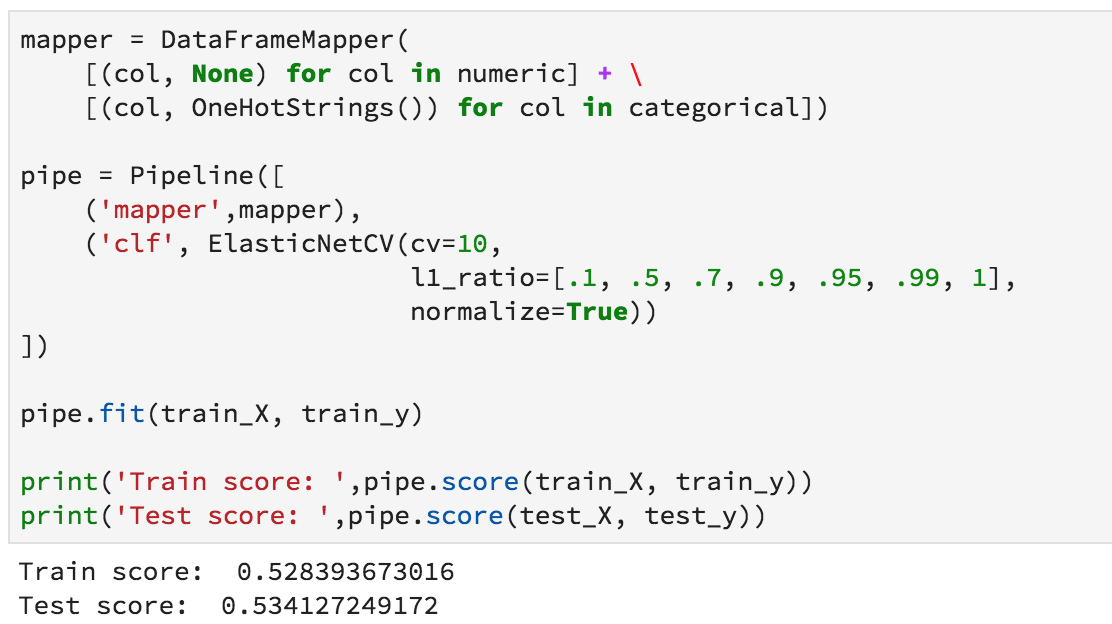
\includegraphics[width=0.55\columnwidth]{../Figures/abalone_map1.png} 
\par\end{center}
\end{frame}

\begin{frame}{Abalone}
\begin{itemize}
	\item $\phi_2(X)$ dummy encodes categoricals and maps numeric features to polynomial features of degree $d \leq 2$.
\end{itemize}
\begin{center}
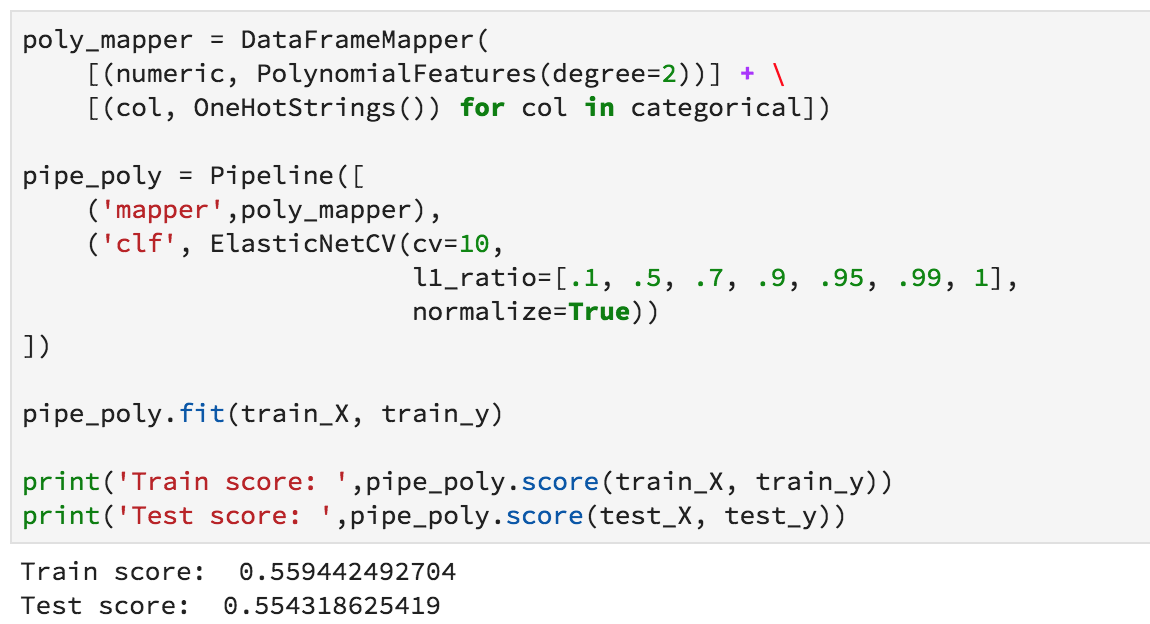
\includegraphics[width=0.55\columnwidth]{../Figures/abalone_map2.png} 
\par\end{center}
\end{frame}


\begin{frame}{Comparing performance}
\begin{itemize}
	\item Why did the performance improve much more for the Boston Housing dataset versus the Abalone dataset when we used map 2?
\end{itemize}
\pause{}
\begin{figure}[H]
    \centering
    \begin{minipage}{.5\textwidth}
        \begin{itemize}
        		\item What is the Bayes prediction function for square loss?
		\pause{}
		\item If $E[Y|X]$ is linear in $\phi_1(X)$, will we improve performance using $\phi_2(X)$?
		\pause{}
		\item Do we typically know in advance the structure of $E[Y|X]$?
        \end{itemize}
    \end{minipage}%
    \begin{minipage}{0.5\textwidth}
        \centering
        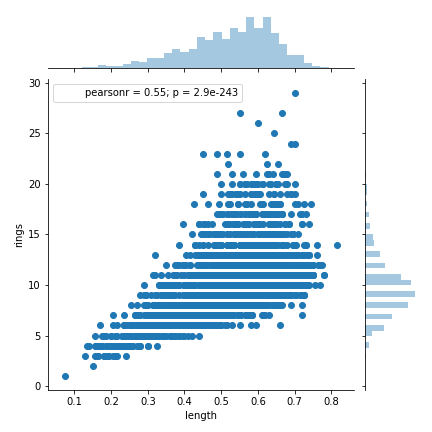
\includegraphics[width=0.7\linewidth]{../Figures/abalone_linear.png}
    \end{minipage}
\end{figure}
\end{frame}

\section{Example 2: Two moons data}

\begin{frame}{Two moons setup}
\begin{center}
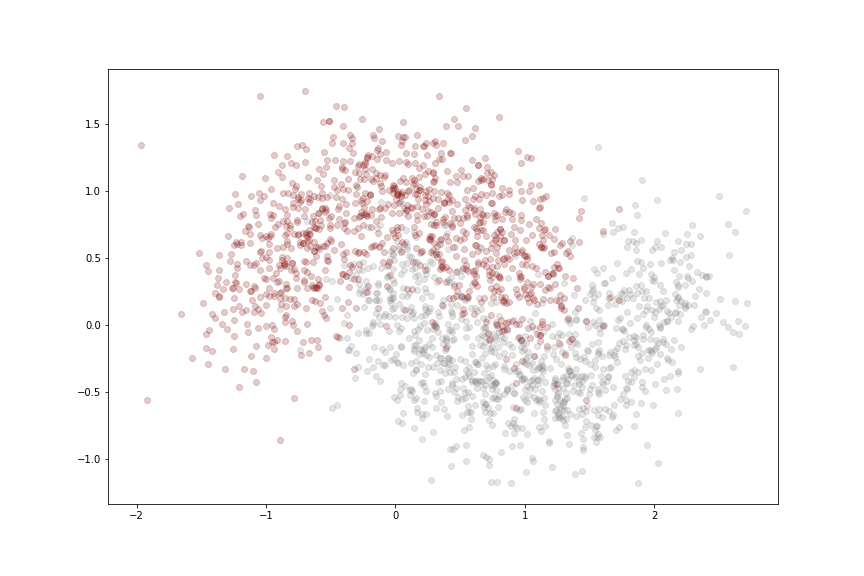
\includegraphics[width=0.45\columnwidth]{../Figures/moons_setup.png} 
\par\end{center}
\begin{itemize}
	\item From Alice Zheng and Amanda Casari's \textit{Feature Engineering for Machine Learning}.
	\item What feature maps might be helpful for this problem?
	\pause{}
	\item We'll try binning data instances using k-means -- let's look at the transformers (\textit{in notebook}).
\end{itemize}
\let\thefootnote\relax\footnotetext{\tiny{See \url{https://github.com/davidrosenberg/mlcourse/blob/gh-pages/Notebooks/Features/vector_quantization.ipynb}}}

\end{frame}


\begin{frame}{Two moons setup}
\begin{itemize}
	\item Here's the pipeline. First, notice the sklearn class \texttt{FeatureUnion}, which let's us easily apply multiple feature maps over an input array.
	\item What is the feature map $\phi(X)$? What will \texttt{transformed.shape[1]} equal?
\end{itemize}
\begin{center}
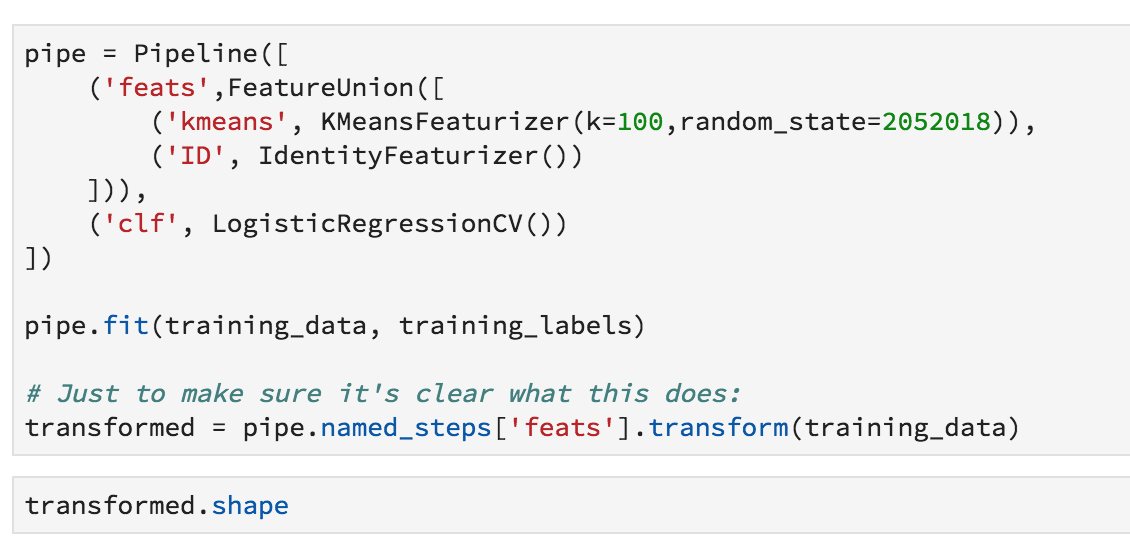
\includegraphics[width=0.6\columnwidth]{../Figures/two_moons_map1.png} 
\par\end{center}
\pause{}
\begin{itemize}
	\item $\phi(X) = \left[X_1, X_2, \mathbbm{1}[(X_1,X_2)\textrm{ binned to centroid 1}], \cdots, \mathbbm{1}[(X_1,X_2)\textrm{ binned to centroid 100}]\right]$
\end{itemize}
\end{frame}


\begin{frame}{Two moons setup}
\begin{itemize}
	\item Here's the pipeline. First, notice the sklearn class \texttt{FeatureUnion}, which let's us easily apply multiple feature maps over an input array.
	\item What is the feature map $\phi(X)$? What will \texttt{transformed.shape[1]} equal?
\end{itemize}
\begin{center}
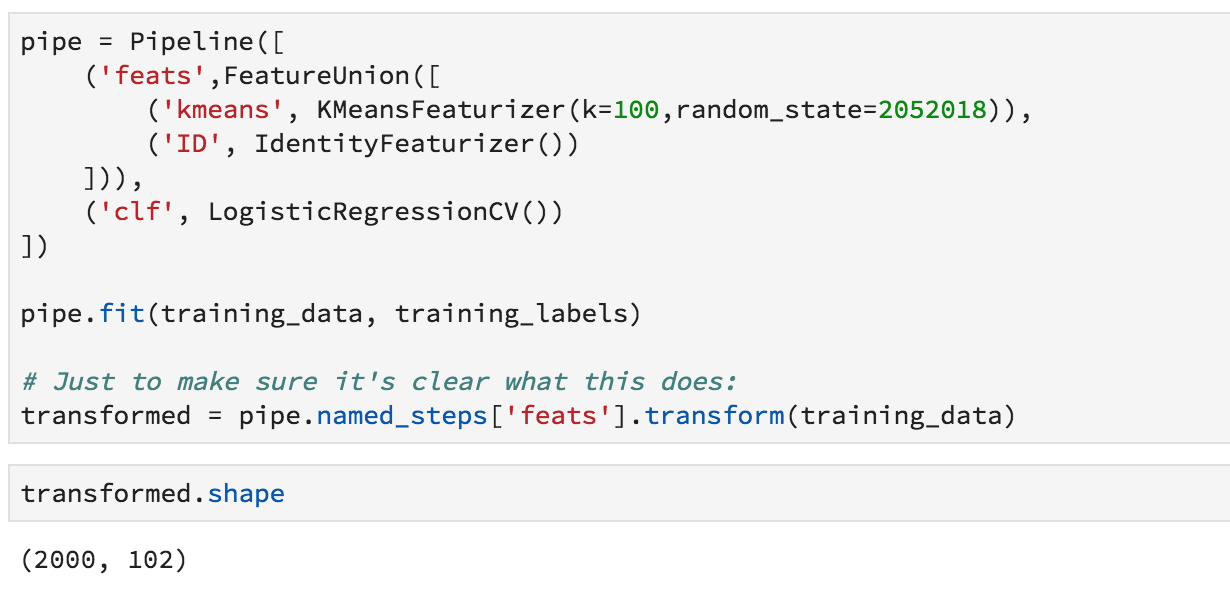
\includegraphics[width=0.6\columnwidth]{../Figures/two_moons_map2.png} 
\par\end{center}
\end{frame}

\begin{frame}{Two moons feature map}
\begin{itemize}
	\item Let's fit this pipe, and compare to a baseline logistic regression over just $\phi_I(X) = X$.
\end{itemize}
\begin{center}
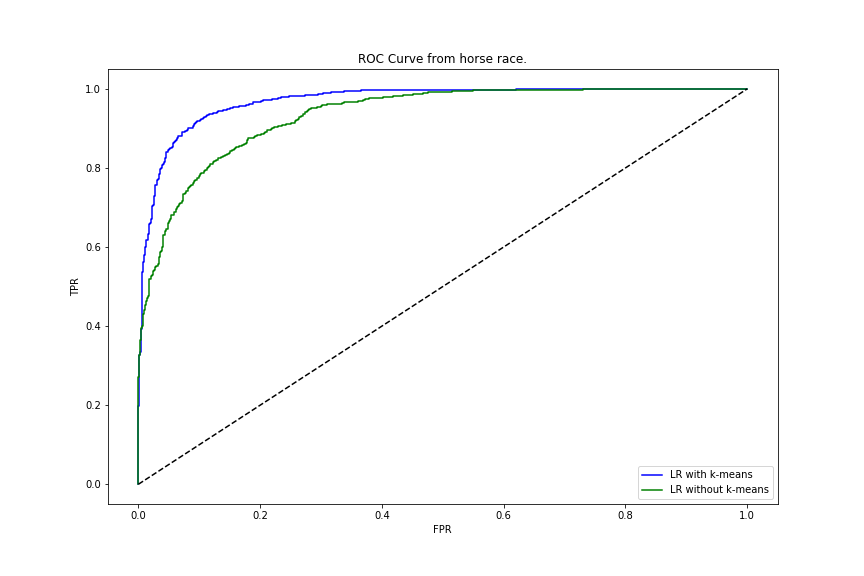
\includegraphics[width=0.5\columnwidth]{../Figures/two_moons_roc.png} \par\end{center}
\begin{itemize}
	\item We see performance improve.
\end{itemize}
\end{frame}

\begin{frame}{Two moons feature map}
\begin{itemize}
	\item Here's the voronoi diagram after fitting the \texttt{KMeansFeaturizer} (fit in \texttt{pipe.fit} call).
\end{itemize}
\begin{center}
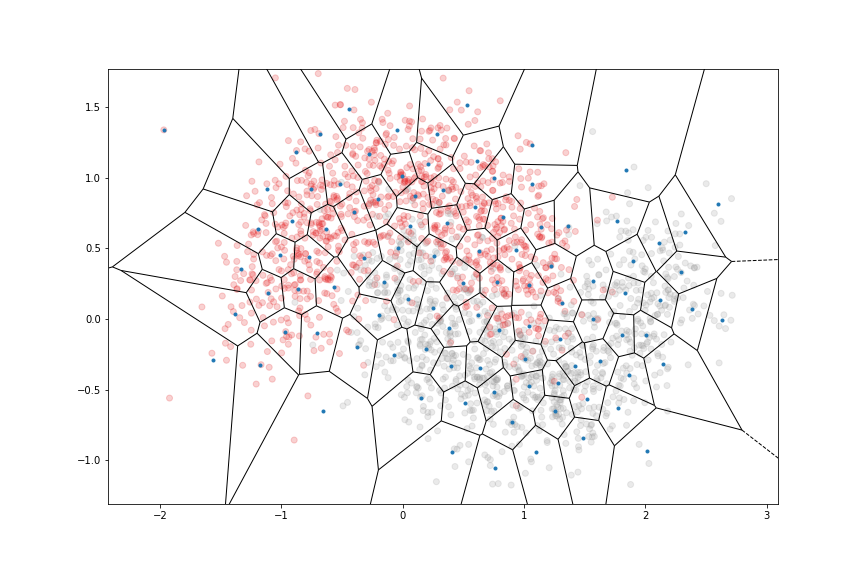
\includegraphics[width=0.5\columnwidth]{../Figures/two_moons_voronoi.png} \par\end{center}

\begin{itemize}
	\item Intuitively, why did this improve performance?
\end{itemize}
\end{frame}

\begin{frame}{Two moons feature map}
\begin{center}
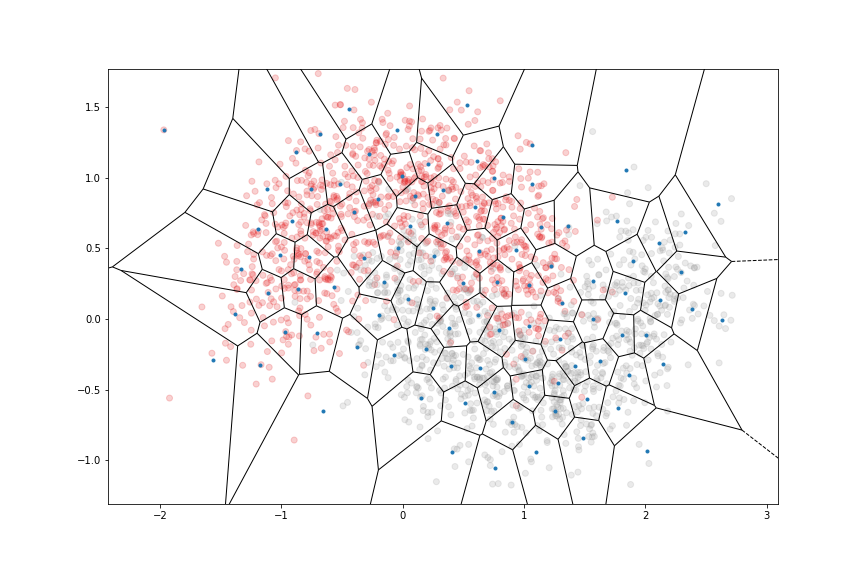
\includegraphics[width=0.5\columnwidth]{../Figures/two_moons_voronoi.png} \par\end{center}

\begin{itemize}
\item Think back to the 1D discretization discussed earlier -- which map is this analogous to?
\end{itemize}
\[
\phi_2(x)=\left(\ind{5\le N(x)<10},\ind{10\le N(x)<100},\ind{100\le N(x)}\right)
\]
\[
\phi_1(x)=\left(\ind{5\le N(x)},\ind{10\le N(x)},\ind{100\le N(x)}\right)
\]
\end{frame}


\begin{frame}{Two moons feature map}
\begin{itemize}
	\item Here's a comparison of decision boundaries (note made using \texttt{mlexend}).
\end{itemize}
\begin{center}
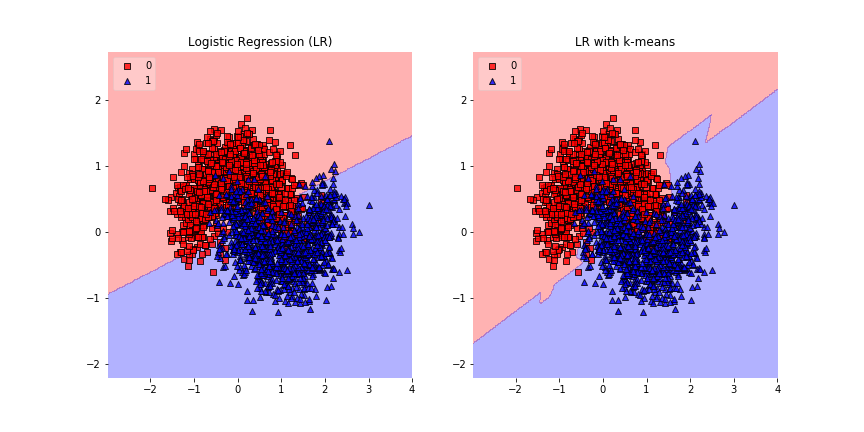
\includegraphics[width=0.7\columnwidth]{../Figures/decision_boundaries.png} \par\end{center}
\begin{itemize}
	\item What's with the plotted decision boundaries? I thought logistic regression was linear?
\end{itemize}
\end{frame}

\begin{frame}{Two moons feature map}
\begin{itemize}
	\item What's with the plotted decision boundaries? I thought logistic regression was linear?
\end{itemize}
\begin{center}
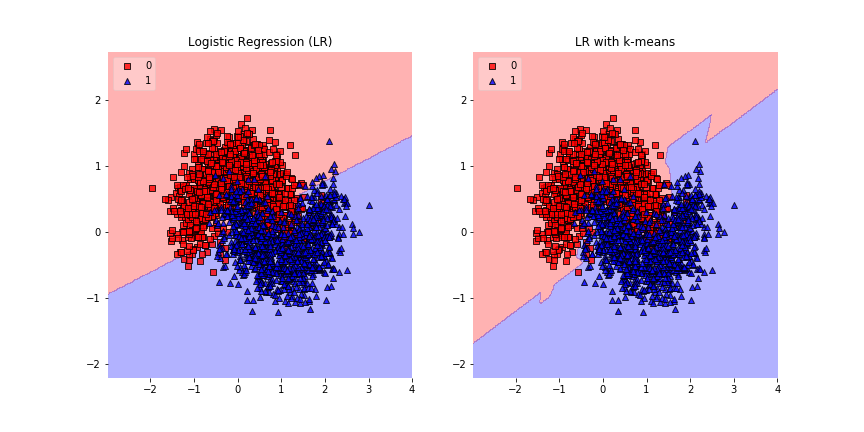
\includegraphics[width=0.7\columnwidth]{../Figures/decision_boundaries.png} \par\end{center}
	\pause{}
\begin{itemize}
	\item Both decision boundaries are affine, but with k-means embedding it's affine in $\reals^{102}$.
\end{itemize}
\end{frame}

\begin{frame}{Learning Objectives}
\begin{itemize}
\item Understand where a \textit{feature map} sits in a machine learning pipeline.
\item Understand that featurization/featuring mapping is inherently required to allow predictors to ingest many types of data.
\item Understand how feature extraction can be used to extend the power of linear methods.
\item Build pipelines with expanded feature spaces using the sklearn ecosystem.
\end{itemize}
\end{frame}

\end{document}


